\documentclass[a4paper, 11pt]{article}
\usepackage{geometry}
\usepackage{amsmath}
\usepackage{subcaption}
\usepackage{graphicx}
\usepackage[table,xcdraw]{xcolor}
\usepackage[some]{background}
\usepackage{lipsum}
\usepackage[utf8]{inputenc}
\usepackage{url}
\def\UrlBreaks{\do\/\do-}
\usepackage{breakurl}
\usepackage[hidelinks, breaklinks]{hyperref}
\usepackage{float}
\usepackage{color}
\usepackage{booktabs}
\usepackage{longtable,lscape}
\usepackage{fancyhdr}
\usepackage[font=small,skip=10pt]{caption}
\usepackage{lscape}
\usepackage{courier}
\usepackage[titletoc,toc,title]{appendix}
\usepackage{listings}
\usepackage{rotating}
\lstset{ %
language=sh,                % choose the language of the code
basicstyle=\footnotesize\ttfamily,breaklines=true,
numbers=left,                   % where to put the line-numbers
numberstyle=\footnotesize\ttfamily, % the size of the fonts that are used for the line-numbers
stepnumber=1,                   % the step between two line-numbers. If it is 1 each line will be numbered
numbersep=5pt,                  % how far the line-numbers are from the code
backgroundcolor=\color{light-gray},  % choose the background color. You must add \usepackage{color}
showspaces=false,               % show spaces adding particular underscores
showstringspaces=false,         % underline spaces within strings
showtabs=false,                 % show tabs within strings adding particular underscores
tabsize=2,          % sets default tabsize to 2 spaces
captionpos=b,           % sets the caption-position to bottom
breaklines=true,        % sets automatic line breaking
breakatwhitespace=false,    % sets if automatic breaks should only happen at whitespace
escapeinside={\%*}{*)}          % if you want to add a comment within your code
}
\definecolor{light-gray}{gray}{0.95}

\usepackage{fancyhdr}

\fancypagestyle{acknowledgements}
{
\fancyhf{}
\renewcommand{\headrulewidth}{1pt}%
\fancyhead[R]{\textsc{Acknowledgements}} % 1. sectionname
\fancyfoot[C]{\thepage}
}

\pagestyle{fancy}
\renewcommand{\sectionmark}[1]{\markboth{#1}{}} % set the \leftmark

\fancyhf{}
\fancyhead[R]{\textsc{\leftmark}} % 1. sectionname
\fancyfoot[C]{\thepage}
\fancypagestyle{plain}{%
  \fancyhf{}%
  \renewcommand{\headrulewidth}{0pt}%

}

%\usepackage{draftwatermark}
%\SetWatermarkText{Draft}
%\SetWatermarkScale{5}

\makeatletter                   
\def\printauthor{%                  
    {\large \@author}}          
\makeatother

\author{%
	\vspace{.25cm}
    \textbf{Siem Hermans} \\
    \texttt{\footnotesize siem.hermans@os3.nl}\vspace{40pt}
    \textbf{Patrick de Niet} \\
    \texttt{\footnotesize patrick.deniet@os3.nl}
    }

\begin{document}
\begin{titlepage}
\newgeometry{bottom=0.5cm}
\begin{center}
  \textbf{\huge Docker Overlay Networks \\}
  \vspace{.3cm}
  \textbf{\large Performance analysis in high-latency environments }
  \\
  \vspace{.5cm}
  
\includegraphics[scale=1.2]{img/UvA-logo-english.jpg}
  \\
  \vspace{.5cm}
  \normalsize \textbf{MSc Research Project}
  \\
  \normalsize System and Network Engineering
  \\
  \vspace{.3cm}
  \normalsize {February 7, 2016}
  \vspace{.2cm}
\end{center}

\begin{figure}[!hb]
  \begin{center}
  	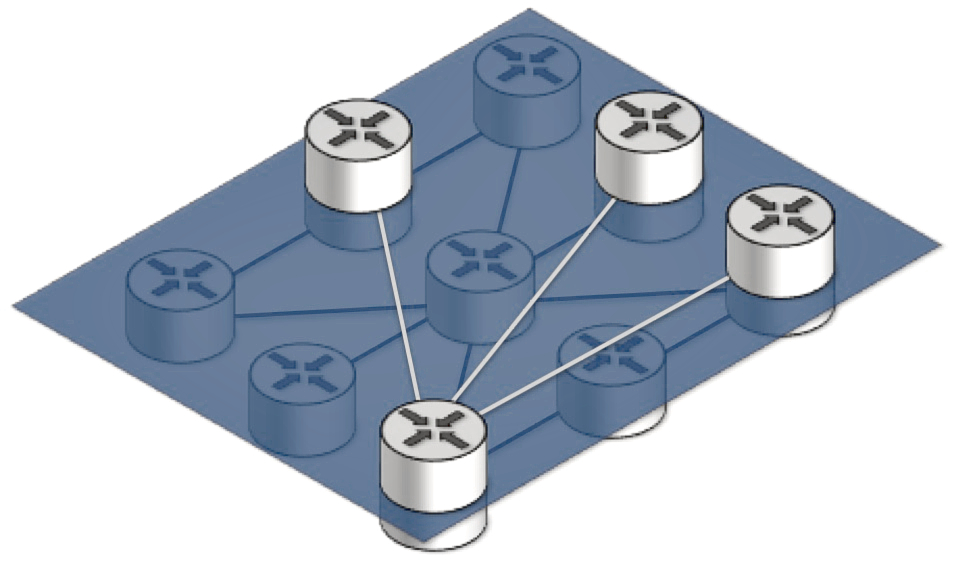
\includegraphics[scale=0.25]{img/cover.jpg}
  \end{center}
\end{figure}

\noindent
\begin{minipage}{0.28\linewidth}
    \begin{flushright}
        \printauthor
    \end{flushright}
\end{minipage} \hspace{8pt}
%
\begin{minipage}{0.02\linewidth}
	\vspace{.67cm}
    \rule{1pt}{181pt}
\end{minipage} \hspace{-26pt}
%
\begin{minipage}{0.80\linewidth}
\vspace{5pt}
    \begin{abstract} 
\footnotesize
\noindent
With the advent of Docker, deploying microservices in application containers has become increasingly popular. The recent incorporation of \texttt{libnetwork} in Docker provides out of the box support for connecting distributed containers via either a native or a third party overlay driver. However, overlay networks introduces an implicit overhead. Additionally, geographic dispersion of containers may have an adverse effect on performance. In this paper, we explore the performance of various Docker overlay solutions when deployed in a high latency environment. We evaluate the deployment feasibility of various overlay solutions in the GÉANT Testbeds Service. Subsequently we measure the performance of the native Docker overlay driver and third party solutions Flannel and Weave via means of a synthetic point-to-point benchmark and a streaming media application benchmark. In either benchmark no significant performance deterioration was identified regarding latency or jitter. UDP and TCP throughput measurements exhibit irregular behavior and require further investigation.    

    \end{abstract}
\end{minipage}
\begin{center}
  \vspace{.8cm}
  \normalsize \textbf{Supervisor:}
  \\
  \normalsize Dr. Paola Grosso
  \\

\end{center}

\end{titlepage}
\restoregeometry

%Table of Contents
\tableofcontents
 
\newpage

%Introduction
\section{Introduction} \label{intro}
Containers, and more specifically Linux containers, have been around for years. Historically, they have been relatively complex to deploy and interconnect on a large scale, which inherently meant that the overall adoption rate has been limited. With the introduction of Docker, the popularity of deploying applications in containers has drastically increased. Docker provides a relatively easy way to to build, ship, and run distributed applications in a uniform and portable manner. An increasing amount of companies have started adopting Docker as an alternative or as a complement to virtualization at a remarkable rate \cite{stackengine_2015}. In contrast with traditional virtualization hypervisors, containers share the operating system with the host machine, which results in a lower overhead, allowing for more containers, and as such, more applications to be deployed. 

The increasing popularity of containerizing applications sparks the need to connect application containers together in order to create (\textit{globally}) distributed microservices. Up until recently this has been a problematic affair as multi-host networking was not natively supported by Docker. However, with the recent introduction of \texttt{libnetwork}, a standardized networking library for containers, Docker offers out of the box support for creating overlay networks between containers whilst allowing third party overlay providers to better integrate with the containers. 

The high density factor of containers and rapid deployment rate require a high performance overlay network which can harness the growing demands. However, as overlay networks are built on top of an underlay network, a performance degradation is implicit. Additionally, deploying applications in geographically dispersed containers may naturally have an adverse effect on performance. Therefore, the aim of this research project is to answer the following main research question:

\begin{quote}
\textit{What is the performance of various Docker overlay solutions when implemented in high latency environments and more specifically in the GÉANT Testbeds Services (GTS)?}
\end{quote}

\noindent
Several sub-questions have been posed to support the main question:

\begin{itemize}
	\setlength\itemsep{1pt}
    \item \textit{Which technical differences exist between the selected Docker overlay solutions?}
    \item \textit{Do performance differences occur when a topology is scaled up in terms of locations and containers?}
    \item \textit{What is the relative performance difference between containers connected through the native \texttt{libnetwork} overlay driver and various third party overlay solutions?}
\end{itemize}

\noindent
The scope of this research is limited by exclusively examining the performance of the native overlay driver and third party solutions Calico, Flannel and Weave. These solutions currently prove to have the most commercial and community backing and are most likely to be deployed in production environments. Lastly, since performance is not the ultimate metric for defining the quality of a solution, the operational flexibility of the technologies is discussed. 

In order to execute performance measurements in a realistic setting, which resembles a network distributed over the internet, the GÉANT Testbeds Service (GTS) has been utilized. This service offers the ability to create experimental networks at scale, geographically dispersed over five European cities. During the course of this project, high latency is defined as a connection with a latency between 10 and 100 milliseconds round trip time. These latencies aim to represent a geographically dispersed environment within Europe. 
\\\\
The rest of the paper is organized as follows. We present the related work in Section \ref{related}, where we provide a brief summary of existing performance evaluations and measurement methodologies. In Section \ref{background} we briefly explain core concepts regarding Docker, \texttt{libnetwork} in general and the selected overlay solutions. The two-part methodology for measuring the performance of the overlay solutions is presented in Section \ref{methodology}. A distinction is made between synthetic benchmarks and a real world scenario. The results, discussion and conclusion are presented in Section \ref{results}, Section \ref{discussion} and Section \ref{conclusion} respectively. 


%Related  Work
\section{Related Work} \label{related}
The performance of Docker containers has been researched in the past multiple times. The main points of interest are usually the differences in performance between traditional virtual machines and containers respectively. For example, Scheepers found that Linux Container (LXC) hypervisors generally outperform traditional hypervisors such as Xen \cite{scheepers2014virtualization}. Soltesz et al. \cite{soltesz2007container} and Morabito \cite{morabitohypervisors} present similar results and show that containers also outperform KVM virtual machines by a fair margin. Furthermore, the performance of applications running in a container versus being directly deployed on a host machine is currently a heavily studied topic. Rohprimardho measured the impact of containerized applications on network I/O performance in a High Frequency Trading (HFT) setting \cite{rohprimardho2015}. He found that the performance degradation of running an application in a container was not significant. He also found that when the configuration of the Docker container was tuned, the performance was identical to applications outside of the container. Other papers focus on the performance implications of various kernel modules in a local environment. Claassen performed an in depth comparison of various kernel modules, used to interconnect containers on a single host. He concludes that for a single host deployment, \texttt{macvlan} in bridge mode poses the best performance. However, in a switched environment there is no significant performance degradation to be found \cite{jorisclaassen2015}. Marmol confirms Claassen's findings and concludes that \texttt{macvlan} and also \texttt{ipvlan} may indeed significantly improve performance \cite{marmolnetworking}. 

All in all, due to their sudden popularity Docker containers are a heavily researched topic. However, at this point in time, little official research has been done on the performance of Docker overlay solutions in general. Claassen briefly investigated overlay solutions and identified Weave, Socketplane and Calico as viable options. However, he concludes on the notion that at the time of writing his paper, the identified overlay solutions weren't production ready yet. Kratzke goes into more detail and examines the performance of containers logically connected by an overlay network on top of virtual machines, which is a common use case in Infrastructure as a Service (IaaS) cloud computing \cite{Kra2015b}. During his research Kratzke exclusively looked at Weave as an overlay solution as he was interested in the performance of an overlay solution with encryption capabilities. In his experiments, Kratzke compares the performance of the Weave overlay with a cross-regional experiment between Amazon Web Services (AWS) regions eu-west-1c (EU, Ireland) and northeast-1-c (Tokyo, Japan). However, the cross-regional experiment exclusively serves as reference material and does not contain an overlay deployment. Kratzke concludes that although containers are seen as lightweight entities, they show a significant impact on network performance. Independent from Kratzke, Michalek saw similar results \cite{lauriemichalek2015} when evaluating the performance of Weave. He found that two containers, networked via Weave provided a mere 6\% of the TCP throughput that two natively deployed services might, at four times the latency. Michalek attributes this performance degradation to the fact that Weave did packet routing in userspace. Important to note is that both Kratzke and Michalek evaluated version 1.1 of Weave. Newer versions perform packet routing based on Open vSwitch (OVS) and provide better integration with \texttt{libnetwork}. As such, they form their opinion on a now outdated version of Weave. 

Due to the recency of Docker introducing \texttt{libnetwork}, most performance analysis have been outdated. Current performance analysis of the selected overlay solutions are mainly to be found in the developer blogs of the respective projects. Each of the selected projects has done their own performance measurements in the past. Flannel's performance measurements are spartan and only report the increase in UDP latency and the decrease in TCP bandwidth when using the overlay. Little is known about the test setup besides the fact that the measurements were done with \texttt{qperf} between two m3.medium virtual machines in Amazon EC2. Yakubovich \cite{1_yakubovich_2014} notes that while Flannel introduces a non-trivial latency penalty, it has almost no effect on the bandwidth. Regarding latency, an increase of over 66\% was examined while TCP bandwidth dropped a mere 1,3\%. Michalek also evaluated Flannel between two entry-level Digital Ocean instances and saw a TCP bandwidth degradation of 3,4\% and a UDP latency increase of 40.52\% \cite{lauriemichalek2015}. However, both of these measurements were performed whilst Flannel was still in an experimental phase meaning that the overall performance may have potentially increased in the past year.


\begin{figure}[!ht]
	\centering
	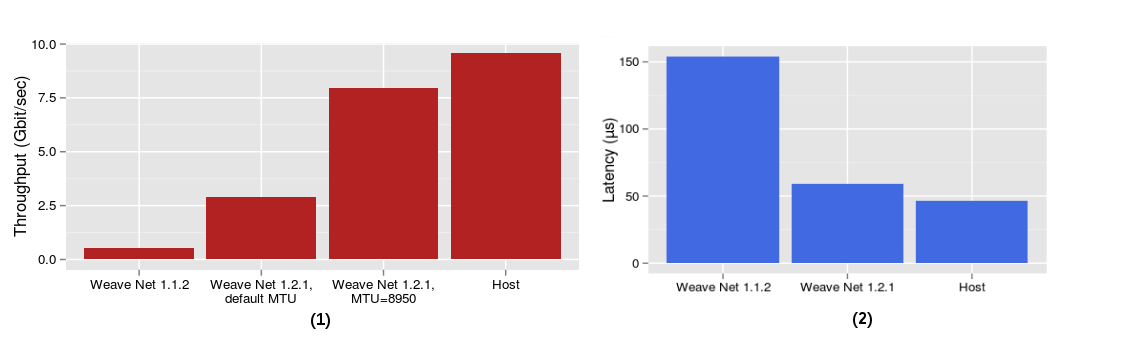
\includegraphics[scale=0.37]{img/weave_perf.png}
	\caption {Performance comparison of Weave versions in terms of throughput (1) and latency (2)}
	\label{fig:weave_perf}
\end{figure}

The developers of Weave and Calico go into more depth and present more detailed results. Wragg \cite{davidwragg2015} evaluated the performance of an older version (1.1) of Weave -which has also been evaluated by Kratzke and Michalek- and the newer version (1.2) which incorporates OVS. Measurements were performed between two Amazon EC2 c3.8xlarge instances \textit{with enhanced networking enabled}. During the experiment, the virtual machines were connected via a 10 Gbps link. Figure \ref{fig:weave_perf} presents the results of the comparison between both Weave versions and native host performance respectively.  Measurements were performed with \texttt{iperf3}. Whilst using the default MTU of 1410 bytes, the performance deterioration of the overall TCP throughput is significant. Wragg attributes these results to a potential bottleneck inside the kernel's network stack. When switching to an MTU size of approximately 9000 bytes (including the VXLAN header) the overall performance is much closer to the performance of the underlying host. He concludes that there is some overhead due to the VXLAN encapsulation which Weave uses, but the results are close to those of host networking. Newer versions of Weave only see a slight decrease in performance and heavily outperform previous versions. Although this performance analysis is executed in a cloud environment, only a single Amazon EC2 availability zone is used. As such, the experiments do not take geographical dispersion into consideration.

White \cite{1_white_2015} presents a performance evaluation of Calico in which he deliberately eliminates the influence of an external network by performing the measurements on two directly connected machines, connected via 10 Gbps interfaces. In this instance the performance is measured with \texttt{qperf}. Figure \ref{fig:calico_perf} presents the results of the throughput and latency measurements. With regards to this research, the bare metal and the container measurements are the main points of interest. Additionally a comparison is made with a standard OpenStack deployment with OVS and VXLAN. The difference in latency between bare metal machines and containers connected with Calico is not significant. However the OVS deployment shows nearly thrice the latency. A similar pattern is seen in the throughput evaluation.   

\begin{figure}[!ht]	
	\centering
	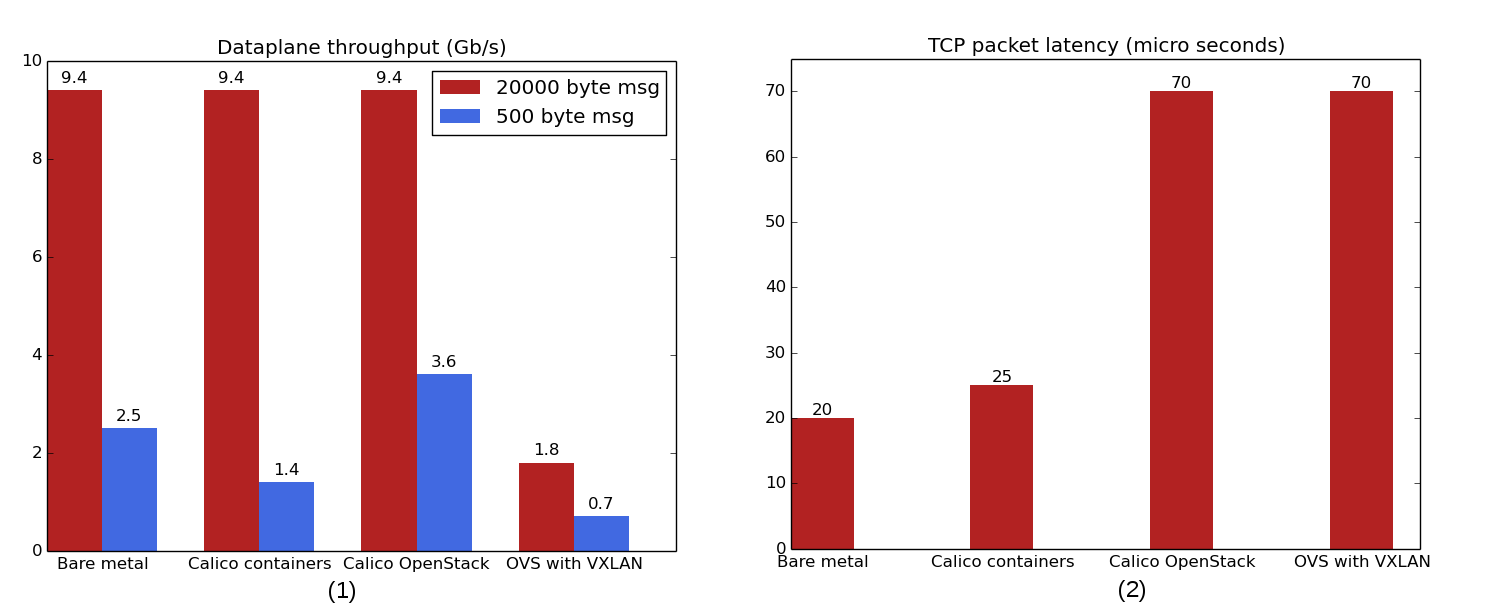
\includegraphics[scale=0.28]{img/calico_perf.png}
	\caption {Performance evaluation of Calico in terms of throughput (1) and latency (2)}
	\label{fig:calico_perf}
\end{figure}

Unrelated to overlay networks, Barker and Shenoy \cite{barker2010empirical} present a series of case studies with which the performance of latency-sensitive applications in a cloud environment can be evaluated. More specifically they present a media streaming setup which resembles a real world scenario. During the course of this project a similar setup will be pursued.

At this point in time, no official research has been performed on the performance of the native overlay driver in \texttt{libnetwork}. Due to the fact that most overlay solutions have restructured their product to work with the modular model of \texttt{libnetwork} nearly all current performance evaluations have become outdated. Moreover, most evaluations exclusively focus on the network performance in a local environment. This paper is a continuation of the work of Claassen and aims to contribute to science by performing a performance analysis of various overlay solutions while factoring in the effects of geographical dispersion. 



%Background Information
\section{Background information} \label{background}
This section presents a brief overview of the inner workings of Docker and explores the technical details of the selected overlay solutions. Moreover, the GÉANT Testbeds Service environment is introduced.  

\subsection{Docker containers \& networking}
Docker is an open platform which aims to make building, shipping (portability), and running distributed applications easier \cite{docker2015}. In order to do so the applications are packaged in a 'container'. A Docker container functions as an execution environment and includes all of the dependencies and libraries required for the application to run. Each container follows a layered model in which layers are added on top of a base image as changes are made to the container. Figure \ref{fig:docker_layers} illustrates an example of this layered structure. On top of the read-only layers a thin read-write layer is shown. Any time a change is made to the running container, the changes are written to this read-write layer. After all changes have been made, the layer can be committed, which creates a new Docker \textit{image}. At that point, new containers can be deployed from the same image. Each container would have the same configuration and state as the container which was used to create the image. Committing layers to an image follows a similar principle as many version control systems employ. 

\begin{figure}[!ht]
   \centering
   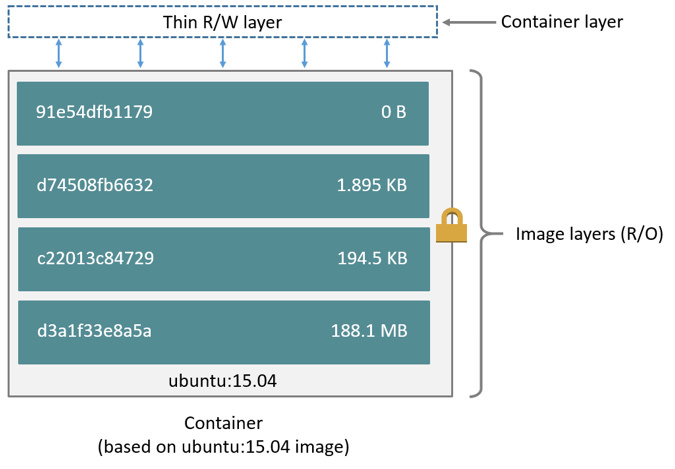
\includegraphics[scale=0.6]{img/container-layers.jpg}
   \caption{Layered model employed by Docker containers \cite{docker2015}}
   \label{fig:docker_layers}
\end{figure}

As with traditional virtualization techniques, containers allow for running multiple isolated user space instances on a single host. However, unlike traditional VMs, they don't require a hypervisor layer to be active on the host machine and instead directly share the kernel with the host machine. \cite{turnbull2014docker}. Furthermore, containers exclusively contain the necessary files to run. This inherently means that containers are lightweight and can start almost instantly. Because containers are so quick to deploy, and because they are deployed in a 'standardized' container format, they lend themselves to building extensive microservices consisting of a multitude of independent building blocks. 

Figure \ref{fig:workflow_docker} illustrates a generic workflow for deploying an application in a container. In the figure, the Docker host is responsible for hosting the containers and maintaining the images. By using the Docker client, the Docker daemon can be instructed to pull an image from the Docker registry. This registry is a centralized repository hosted by Docker, containing a large collection of official Docker images. This application can be a pre-packaged application image, which in turn can directly be deployed in a new container.

\begin{figure}[!ht]
   \centering
   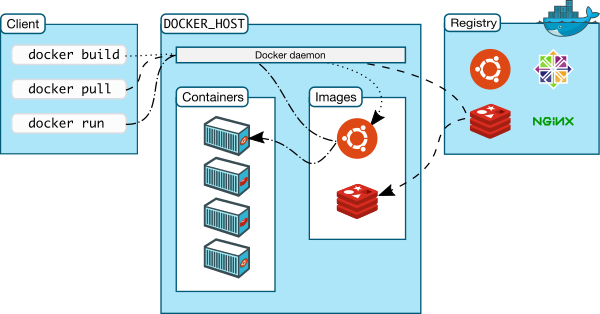
\includegraphics[scale=0.45]{img/architecture.png}
   \caption{Workflow for deploying applications to Docker containers \cite{multihost2015}}
   \label{fig:workflow_docker}
\end{figure}

The image illustrates how a Redis application is deployed in a single Ubuntu container. Docker was originally developed to improve the application development process. Docker allowed developers to build an entire multi-tier application on a single Linux workstation without the complexity or overhead of multiple operating system images \cite{techrepublic2015}. Because all containers were initially hosted on a single machine, Docker used a rather simple networking model. By default, Docker used private networking to connect containers via a special virtual bridge, \texttt{docker0}. This bridge was allocated a subnet from a private IP range. In turn, every deployed container was given a virtual Ethernet interface (usually abbreviated to 'veth' interface) which was attached to the \texttt{docker0} bridge. From inside of the container, the veth interface appeared as a regular \texttt{eth0} interface by using Linux namespaces. Each of the veth interfaces was addressed by the \texttt{docker0} bridge in the same private subnet. As a result, the containers were able to communicate with each other when they were located on the same physical machine and shared the same bridge interface. Prior tot Docker version 1.9, communicating with containers on other hosts was difficult. In order for the containers to communicate with each other they had to be allocated a static port on the hosting machine's IP address. This port number was then forwarded to other containers. Inherently this meant that hosting a cluster of web servers on a single node was difficult, as ports were statically mapped to specific containers. Connecting containers required a lot of coordination and planning. 

By linking containers with static ports, the overall configuration used to be relatively static. Moving containers between hosts required reconfiguration and portability was limited. Third party overlay projects were aiming to alleviate system administrators from static network configurations by connecting the containers via an an allocated IP address in an overlay network. Overlay networks allow for dynamically creating logical links between endpoints which have no coupling to the hardware infrastructure of the underlay network, effectively abstracting out the physical network. This meant that all containers in the overlay network could communicate with each other, regardless of their host placement or the IP address of the host machine. As such, containers do not have to be statically linked anymore based on a port number. However, early overlay solutions had to wrap around the Docker API as multi-host networking was not supported out of the box.

\subsection{Libnetwork}
The Docker team recognized the problem of connecting containers and as of version 1.9, \texttt{libnetwork} is included in the main release of the project. The idea behind \texttt{libnetwork} is to replace the networking subsystem that was in place in previous versions of the Docker Engine with a model that allows local and remote drivers to provide networking to containers. This means that Docker’s full networking code has now been included in a separate library called “\texttt{libnetwork}”. Docker achieved their modular ideal by implementing the Container Network Model (CNM). The premise of the CNM is that containers can be joined to networks in a multitude of ways and based on their configuration, all containers on a given network can communicate with each other \cite{5_bridgen_2015}. Previously, due to the static port bindings this proved to be difficult. With the introduction of CNM, Docker aims to address containers more like standalone hosts when they are deployed in overlay mode.

The innovation of the network stack was kickstarted when Docker acquired the SocketPlane team in March 2015 \cite{socketplane2015}. SocketPlane was one of the many available Software-Defined Networking solutions for containers on the market. Instead of connecting to a virtual bridge, each container would connect to an Open vSwitch (OVS) port. Each container host would have an OVS instance running which allowed them to form a virtual overlay network that would carry traffic destined for any container connected to the network via VXLAN. This allows containers to seamlessly communicate with each other wherever they are and thus enabling true distributed applications \cite{multihost2015}. 

\begin{figure}[!ht]
   \centering
   \includegraphics[scale=0.5]{img/cnm_model.png}
   \caption{Visual representation of the Container Network Model \cite{GITHUB}}
   \label{fig:cnm_model}
\end{figure}

The CNM relies on three main components: the sandbox, endpoints and networks. Figure \ref{fig:cnm_model} presents a visual representation of the three components placed in the model. In essence, the model is relatively simple. A (network) sandbox contains the configuration of a container's network stack. This includes management of the container's interfaces, routing table and DNS settings \cite{GITHUB}. As would be the case with a standard virtual machine, a sandbox can have multiple endpoints attached to a multitude of different networks. This is also illustrated in figure \ref{fig:cnm_model}. The middle container has two endpoints connected to two different networks. In turn, an endpoint connects a sandbox and thus a container to a network. A real world implementation of an endpoint could be a veth pair or in the case of various overlay solutions and Open vSwitch port for example. Docker defines a network in the CNM as "a group of Endpoints that are able to communicate with each-other directly" \cite{GITHUB}. An implementation of the network component could be a bridged network interface or a VXLAN segment.

Although Docker is the first containerization project to implement the model, CNM is a generic model that does not only apply to Docker exclusively, and can also be implemented in more traditional container projects like OpenVZ and LXC. By employing a modular model, \texttt{libnetwork} functions as a common ground for other overlay solutions. SocketPlane was only one of the available solutions on the market. Competing vendors and projects that can be identified are Calico, Flannel and Weave \cite{jorisclaassen2015}. As such there are many networking solutions available, suited for a large set of diverse use-cases. In order to standardize how containers are networked, \texttt{libnetwork} employs a driver plug-in model which allows third party solutions to plug directly into the Docker Engine. The end user on the other hand is only exposed to a consistent Network Model. The CNM abstracts the complexity of the third party plug-ins. For third party solutions, CNM provides a consistent programming interface which makes integrating with the Docker networking stack easier than in the past. 

The driver is the most abstract component of \texttt{libnetwork} and is not a user visible object. Drivers provide the actual implementation that makes the network work. By default Docker provides four drivers: a null, bridge, overlay and remote driver. The most commonly used driver is the 'bridge' driver. The bridge driver allows for single-host communication between containers by using Linux Bridging and iptables for segmentation. This driver is discussed in detail in Claassen's paper \cite{jorisclaassen2015}. The overlay driver is based on SocketPlane and implements networking that can span multiple hosts using VXLAN. Third party providers make use of the 'remote' driver. Build-in drivers such as 'bridge' and 'overlay' register inside of \texttt{libnetwork}, while remote drivers register with \texttt{libnetwork} via the plugin mechanism. 

\subsection{Third party overlay solutions}
During the course of this project we focus on the overlay solutions Calico, Flannel and Weave. Table \ref{overlayschar} presents a quick overview of the technical differences between the selected solutions. The successive subsections will to into more detail about each individual product.   

\begin{table}[H]
\centering
\begin{tabular}{@{}ll@{}}
\toprule
\textbf{Native overlay} & \textbf{Weave Net} \\ \midrule
Native integration & Libnetwork plug-in \\
VXLAN forwarding & VXLAN forwarding \\
Dedicated key-value store (any) & No dedicated key-value store (CRDT) \\
 &  \\ \midrule
\textbf{Flannel} & \textbf{Project Calico} \\ \midrule
No integration & Libnetwork Plugin \\
UDP or VXLAN forwarding & BGP routing \\
Dedicated key-value store (etcd) & Dedicated key-value store (any) \\ \bottomrule
\end{tabular}
\caption{Overlay solution characteristics}
\label{overlayschar}
\end{table}


\subsubsection{Weave}
Weave provides a Docker overlay solution named 'Weave Net'. Weave overlay consists of a multitude of Weave routers. Such a software router is placed on every machine participating in the overlay. In practice, this means a Weave container is launched within Docker. In addition to this container, a bridge interface is created on the host itself. In turn, containers within the overlay (including the Weave router) connect to this bridge using their veth interface which is supplied an IP address and subnet mask by Weave’s IP address allocator \cite{Weave2015}. As discussed in Section \ref{related}, Weave made use of \texttt{pcap} to route packets in previous versions of the project. However, as all packets had to be moved to userspace, this resulted in a significant performance penalty. In addressing this issue, Weave has added 'Weave Fast Datapath' in Weave version 1.2, which utilizes Open vSwitch \cite{davidwragg2015}. This allows Weave Net to do in-kernel routing which allows for significantly faster routing of packets between containers. Weave Router peers communicate their knowledge of the topology (and changes to it) to other routers, so that all peers learn about the entire topology. 

To application containers, the network established by Weave looks like a giant Ethernet switch to which all the containers are connected. In version 1.2, Weave was developed as a plug-in to \texttt{libnetwork}. As such, the Weave Net plugin actually provides two network drivers to Docker - one named \texttt{weavemesh} that can operate without a cluster store, and one named \texttt{weave} that can only work with one. By default \texttt{weavemesh} is utilized. As with all other overlays, Weave works alongside Docker's existing bridge networking capabilities which means that single-host communication is still possible without using Weave. In version 1.2, Weave still allows for \texttt{pcap} based routing when it is needed in specific scenarios. By default, Weave chooses their newly introduced Fast Datapath method (\texttt{fastdp}). However, when packets have to traverse untrusted networks and require encryption, the slower 'sleeve’ mode is used. At this point in time Weave can not provide encryption when using \texttt{fastdp} \cite{9_wragg_2015}.


%Weave creates a network bridge on the host. Each container is connected to that bridge via a veth pair, the container side of which is given an IP address \& netmask supplied either by the user or Weave’s IP address allocator. Also connected to the bridge is the weave router container. Weave routers learn which peer host a particular MAC address resides on. They combine this knowledge with topology information in order to make routing decisions and thus avoid forwarding every packet to every peer. Weave can route packets in partially connected networks with changing topology. Project Calico on the other hand utilises BGP for routing between containers and aims for extreme scalability.

%The topology information captures which peers are connected to which other peers. Weave peers communicate their knowledge of the topology (and changes to it) to others, so that all peers learn about the entire topology. This communication occurs over the TCP links between peers, using a) spanning-tree based broadcast mechanism, and b) a neighour gossip mechanism.

%Open vSwitch can operate both as a software-based network switch running within the virtual machine (VM) hypervisors, and as the control stack for dedicated switching hardware

%To application containers, the network established by weave looks like a giant Ethernet switch to which all the containers are connected.

%The Weave Net plugin actually provides two network drivers to Docker - one named weavemesh that can operate without a cluster store (like Docker’s overlay driver) and one named weave that can only work with one.

%Weave creates a virtual network that connects Docker containers deployed across multiple hosts and enables their automatic discovery. Weave works alongside Docker's existing (single host) networking capabilities, so these can continue to be used by containers.

%Fast data path reduces CPU overhead and latency because there are fewer copies of packet data and context switches. The packet goes straight from the user’s application to the kernel, which takes care of adding the VXLAN header (the NIC does this if it offers VXLAN acceleration).

%\begin{figure}[!ht]
%   \centering
%   \includegraphics[scale=0.42]{img/weave_userspace.png}
%   \caption{Weave datapath structure}
%   \label{fig:gts_env}
%\end{figure}

%In any case where Weave can’t use fast data path between two hosts it will fall back to the slower packet forwarding approach used in prior releases. The selection of which forwarding approach to use is automatic, and made on a connection-by-connection basis. So a Weave network spanning two data centers might use fast data path within the data centers, but not for the more constrained network link between them.

%Weave automatically chooses the fastest available method to transport data between peers. The most performant of these ('fastdp’) offers near-native throughput and latency but does not support encryption; consequently supplying a password will cause the router to fall back to a slower mode ('sleeve’) that does, for connections that traverse untrusted networks


\subsubsection{Flannel}
Flannel is another third party solution aimed towards building overlays between Docker hosts. The solution is part of CoreOS' product portfolio. Whereas Weave and Calico deploy separate container instances to manage the network, Flannel creates an agent, flanneld, on each container host which controls the overlay. All services are kept in sync via a key-value store.

The containers and their physical hosts are stored in the \texttt{etcd} datastore which is also created by CoreOS itself. Containers are assigned IP addresses from a pre-defined subnet, which is stored in the key-value store. Other than the alternative overlays, Flannel currently does not offer integration with the \texttt{libnetwork} plugin. However, representatives have noted it may very well be included later \cite{newsgroups_2015}. By default Flannel uses UDP tunneling to connect containers. In newer versions however VXLAN forwarding with Open vSwitch has been introduced to increase the performance of the overlay solution \cite{flannel_2015}.

As Flannel was built for Kubernetes, the solution  offers tight integration with the open source container cluster manager by Google. Kubernetes is aimed at large scale environments with a multitude of containers \cite{1_yakubovich_2014}.

\subsubsection{Calico}
Project Calico is technically not an overlay network but a pure layer 3 approach to virtual networking. Although we primarily evaluate overlay solutions, it is still worth mentioning because Calcio strives for the same goals as overlay solutions. The idea behind Calico is that data streams should not be encapsulated, but routed instead. This is achieved by deploying a BIRD Internet Routing Daemon on each container host. Calico uses the Border Gateway Protocol (BGP) as its control plane to advertise routes to individual containers across the physical network fabric \cite{calicosource}.

As with Flannel and Weave, every container is assigned its own IP address from a pre-defined pool. As Calico does not connect containers via tunneling techniques, segmentation between containers is achieved by modifying the \texttt{iptables} configuration of the host machine. Effectively, Calico functions as a firewall between network segments.

All traffic between containers is routed at layer 3 via the Linux kernel’s native IP forwarding engine in each host. This means that no overhead is imposed when containers try to communicate. No additional encapsulation headers are added. Like Weave, Calico functions as a \texttt{libnetwork} plug-in. The Calico network is controlled by a series of Docker containers, managed by the \texttt{calicoctl} tool which exchange state information via the BGP routing instances. State exchange of the network is achieved with BGP route reflectors

\subsection{Key value stores}
One dependency almost all overlay solutions share is the utilization of a Key-Value (KV) stores. This NoSQL datastore is used to create a key-value database to which the overlays technologies write their data. While the exact way the datastore is used differs slightly per overlay technology, generally the values stored are related to global IP address allocation and node discovery. In some cases additional information such as container names are also stored. Weave uses it's own proprietary storage system based on the 'Conflict-free Replicated Data Type' (CRDT) principle, as they believe this is best for the availability of the overlay \cite{7_richardson_2015}. The other technologies support a variety of KV-stores which are 'Consensus-Based' (CB). One example of an open-source CB datastore is \texttt{etcd}, which is the only datastore supported by all overlay technologies we will be using (Weave excluded). If any of the datastore-systems were to malfunction, the following effects would occur:

\begin{itemize}
  \item Inability to create new overlay networks;
  \item Inability to allocate global IP addresses;
  \item Inability to add a container to the overlay.
\end{itemize}

For the purposes of measuring the overlay performance, these implications are unrelated and not an issue. This is due to the fact that we are working with a fixed environment and are testing performance rather than availability.
Once the overlays and containers required for testing have been created and added to the KV store, the datastore will be idle. This means that the datastores used and their respective configurations are of no consequence to this project.

%\texttt{etcd} is a product of CoreOS

%Docker Networking in 1.9 requires an external Key-Value (KV) store, which is used for global IP address allocation and node discovery. The store is accessed via an API, libkv, that is advertised as working with Consul, etcd, and ZooKeeper.

%Essentially this means you have to install an additional distributed system in order to set up networking, for each Docker cluster, may not be to everyone’s taste. Scalability issues come into play when the amount of hosts in the KV store is extended beyond 5 to 10 hosts. Root cause analysis is harder: Figuring out whether bugs are in the application, or in Docker networking, or the external KV store, is up to you.

%Using the built-in network drivers in Docker 1.9 requires that a consistent KV store is visible from all Docker hosts. In practice however this either means a) having the KV cluster in one of the data centers, introducing a SPOF or b) spreading the KV cluster across multiple data centers, greatly increasing the likelihood of transient partitions and hence quorum failure (with results as above)

%All other Docker networking plugins, including Docker’s own “Overlay” driver, require that you set up Docker with a cluster store – a central database like Consul or Zookeeper – before you can use them. As well as being harder to set up, maintain and manage, every Docker host must be in constant contact with the cluster store: if you lose the connection, even temporarily, then you cannot start or stop any containers.

%All cross-host coordination is handled by Weave Net’s “mesh” communication, using gossip and eventual consistency to avoid the need for constant communication and dependency on a central cluster store.

\subsection{GÉANT Testbed Services} \label{gts_sec}
In order to do performance measurements in a realistic setting, which resembles a network distributed over the internet, the GÉANT Testbeds Service (GTS) will be utilized. This service offers the ability to create experimental networks at scale, geographically dispersed over five European cities. Figure \ref{fig:gts_env} presents a high-level overview of the GTS environment. GÉANT is a European research network which focuses on services aimed at research and education. GÉANT has Points of Presence (PoPs) in Amsterdam, Bratislava, Ljubljana, Milan and Prague. The sites are connected via dedicated point-to-point circuits 10 Gbps optical waves in an Multi Protocol Label Switching (MPLS) cloud.

The GTS physical infrastructure is assembled into a set of equipment pods which contain the hardware components that make up the virtual machines, virtual circuits and other resources. Figure \ref{fig:gts_env} presents a high level overview of the GTS infrastructure. All locations provide equal capabilities for provisioning (virtual) machines and provide equal connectivity. The virtual machines in GTS are deployed in Kernel-based Virtual Machine (KVM) by OpenStack. Each VM uses \texttt{pci\_passthrough}, giving it full and direct access to the network interface card (NIC) of the host machine. All virtual machines are deployed with Ubuntu 14.04 LTS by default.

\begin{figure}[!ht]
   \centering
   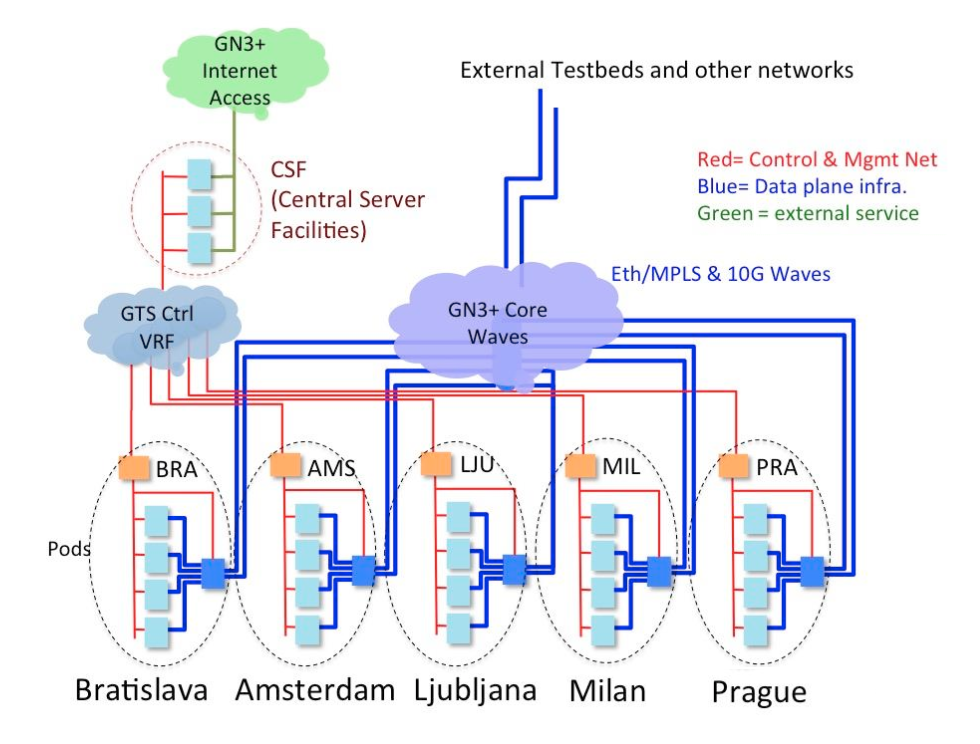
\includegraphics[scale=0.32]{img/gts_env.png}
   \caption{The GTS distributed architecture across the GÉANT core network}
   \label{fig:gts_env}
\end{figure}

Each testbed created in the environment forms an isolated (virtual) environment which shares resources with other users of the service. As such, interference with other projects running within GTS is to be expected and cannot (and should not, for the purposes of this project) be avoided. This way generic Internet traffic is resembled. Preliminary tests in the testbed service have shown latencies between the PoPs ranging between 15 ms and 60 ms which falls within our definition of high latency as presented in Section \ref{intro}.



%Method
\section{Methodology} \label{methodology}
In order to evaluate the performance implications of geographic dispersion on the overlay solutions, a high latency simulation environment is required. As previously discussed in section \ref{gts_sec}, we have utilized the GÉANT Testbeds Service for this purpose. Within this service, entire topologies can be created using a domain-specific language (DSL) which follows a JSON formatting. The DSL description defines the structure of the topology and the properties of each requested resource, i.e. the required attributes of the resource. The deployment application programming interface (API) hooks into GÉANT's OpenStack environment and provisions the underlying technologies based on the provided DSL file. Listing \ref{dslexample} presents a snippet of a basic point-to-point topology in GTS. 
\\
\begin{lstlisting}[caption={DSL example illustrating a simple host resource definition},label=dslexample]
FullMesh {
	id="FullMesh_Dispersed"
	host { id="h1" location="AMS" port {id="port11"} port {id="port12"} }
	link { id="l1" port {id="src"} port {id="dst"} }
	adjacency h1.port14, l1.src
	adjacency h2.port24, l1.dst
} {...}
\end{lstlisting}

In order to form an adjacency between hosts, links have to be statically defined in the JSON schema and associated with a port on the host object. During the course of the project the third version of GTS has been rolled out (v3.0.1). The new version of GTS introduced 'second generation' networks which allow for more advanced configurations and dynamic in-site modification. For example, the ability to modify an active topology without tearing down the entire existing testbed instance and the characteristics of resources can be specified in more detail. However, at the time of writing, the documentation on the newly introduced features in the DSL is not available yet. This means that our topologies in GTS are defined using the older v2.0 DSL constructs. In practice this means that the topologies are dynamically provisioned but remain static throughout their reservation. Changes in the topology require tearing down the entire testbed before reserving it again. Due to this limitation we have opted to create an as flexible as possible topology within GTS: a full mesh topology between all sites. 

Using the DSL we defined the full mesh topology and deployed it to a total of four instances in GTS, one for each of the overlay solutions to be tested. A full mesh topology was primarily chosen to make measuring the performance as flexible as possible seeing as a full mesh allows for a multitude of potential test scenarios. During the course of the project we have divided the full mesh in a series of point-to-point topologies and a star topology. Due to the software-based nature of an overlay, a full mesh would be a feasible topology in a real world scenario. Lastly, a full mesh was preferable because Calico utilizes the Border Gateway routing protocol (BGP) to route traffic through the network. Due to this property the solution may potentially utilize unequal cost load balancing which would benefit from redundant paths. 
\\ \\
At first an instance of the full mesh topology was deployed in a single site in GTS to assess the deployment feasibility of the selected overlay solutions. The full results of this assessment are presented in Section \ref{results}. After the initial feasibility validation, the topology was scaled out to all available sites in GTS and overlay networks were created in each instance. Figure \ref{fig:gts_topology} is a visual representation of the full mesh as defined in the DSL file. Each host is directly connected via their network interfaces to all other hosts. 

\begin{figure}[!ht]
   \centering
   \includegraphics[scale=0.64]{img/mesh.png}
   \caption{Full mesh topology between all sites in GTS}
   \label{fig:gts_topology}
\end{figure}

It should be noted that during the course of the project, the virtual machines deployed in the Prague site have become unresponsive for an extensive period of time. This means that the Prague site has not been taken into consideration whilst measuring the performance, effectively reducing the topology to a four-node mesh. Additionally, because we make use of the GTS v2.0 DSL grammar, the placement of the virtual machine on a specific physical host cannot currently be controlled with the DSL and are as such, assigned by OpenStack based on available resources. This means that it is very well possible that all four nodes in Amsterdam (one per instance) are placed on the same physical host. While in Milan, each node is placed on a separate physical host. If we would run all performance measurements simultaneously, a discrepancy unrelated to the actual functioning of the overlays can be expected. To avoid this external influence, the tools will be timed and scheduled to ensure no two distinct hosts are running simultaneously. A detailed explanation of this procedure can be found in section \ref{tools}.

Additionally, due to the way the virtual machines are provisioned in GTS, it is infeasible to create a fully functional meshed topology as depicted in figure \ref{fig:gts_topology} with Calico. The BIRD routing daemon, which lies at the core of Calico, refuses to import a route from the kernel if the next-hop is not in a directly connected network. This essentially means that only physically connected networks can be included in the routing table as a correct BGP route, effectively limiting the topology to a point-to-point link. A workaround in order to include the links that are not directly connected to the routing table would be to issue a route to the link and specify the route as \texttt{'onlink'}. By issuing this next hop flag (\texttt{NHFLAG}) with the \texttt{ip} command, the networking stack will pretend that the next-hop is directly attached to the given link, even if it does not match any interface prefix. The \texttt{NHFLAG} parameter essentially instructs the kernel to treat the route as a connected network. However, specifying this flag in the GTS returns that the \texttt{NHFLAG} is an invalid argument for the specified virtual interface. Moreover, whilst attempting to create a point-to-multipoint topology, forming adjacencies between the shared node failed. This means that Calico's overlay solution is limited to point-to-point topologies between sites in GTS specifically. Because Calico is not suited for all desired test cases in GTS, we have have opted to drop this solution from the performance measurements. 

\subsection{Deployment considerations}
Disregarding the local site topology, each of the deployed instances houses one of the selected overlay solutions. Due to the large amount of instances and nodes per instance, a bootstrap script has been created which handles basic machine configuration tasks and automates the deployment of Docker. Furthermore, if desired, the script also performs the installation and configuration of one of the respective third-party overlay solutions. For quick reference, all created scripts have been made available on GitHub \footnote{All configuration scripts are made available at \url{https://github.com/siemhermans/gtsperf}}. 

The configuration of the overlay solutions has been kept default as much as possible. Still, some deployment specific choices have been made. Flannel for example has been configured to utilize in-kernel VXLAN to encapsulate the packets. By default Flannel used UDP encapsulation to tunnel packets between containers. Because both the native overlay driver and Weave use VXLAN out of the box, we have opted to make Flannel use VXLAN as well. This has been achieved by setting a specific value in the \texttt{etcd} store. 

\begin{lstlisting}[caption={Configuring Flannel to use VXLAN instead of UDP tunneling},label=flantun]
etcdctl set /coreos.com/network//config  '{ 
	"Network": "10.1.0.0/16", "Backend": { 
    	"Type": "vxlan"
    } 
}'
\end{lstlisting}

Regarding the key-value store, both Flannel and the native Overlay driver require a dedicated key-value store to hold information about the network state. As Flannel is a product of CoreOS, this overlay natively works with \texttt{etcd}. In order to maintain a homogeneous environment, \texttt{etcd} has been used for all overlays which require a key-value store. The Amsterdam site has been selected to house the \texttt{etcd} instance. In a real world scenario it would be desirable to deploy the key-value store as a distributed system in itself. However, due to the fact that process resilience is of lesser importance during this project we have opted to deploy a standalone instance of \texttt{etcd} without any clustering. As previously discussed, the key-value store is only used by containers to register their service and by the overlays to store the network state. As such, \texttt{etcd} doesn't negatively affect performance. Because Weave utilizes an eventually consistent distributed configuration model (CRDT), no key-value store is required for this particular overlay.

Lastly, no specific configuration steps have been taken to integrate the overlay solutions with \texttt{libnetwork}. Current versions of Weave automatically run as a plugin, given the Docker version on the system is 1.9 or above. This means that Weave does not function as a wrapper to the Docker API anymore but gains more native integration. As Flannel works separately from \texttt{libnetwork}, this overlay has been tested as a standalone. Implicitly, the native overlay driver exclusively functions as a plug-in to \texttt{libnetwork}. Since the native overlay driver requires a kernel version of at least 3.16, we have upgraded all machines in GTS from their default 3.13 kernel to version 3.19 with the bootstrap script. 

\subsection{Measurement tools} \label{tools}
To measure the performance, \texttt{iperf} and \texttt{netperf} are used. These tools are both industry standard applications for benchmarking connections and are used in a multitude of scientific papers \cite{rohprimardho2015}, \cite{jorisclaassen2015}, \cite{Kra2015b}, \cite{barker2010empirical}. During our research \texttt{iperf} is primarily used to measure the UDP and TCP throughput, while \texttt{netperf} is primarily used to measure the latency between sites and the effect of employing an overlay solution on the overall latency. While \texttt{iperf} could technically be used to measure latency, \texttt{netperf} provides more detailed statistics out of the box. Furthermore we are interested in the potential jitter introduced by each overlay solution. Here, jitter refers to the variability in delay between receiving packets. Naturally, a connection with irregular intervals will have an undesirable amount of jitter which may be disruptive for latency sensitive applications. We have opted not to tune the measurement tools (e.g. the TCP window size or segment sizes), as we are merely interested in the relative performance difference between the overlay solutions. Whilst measuring the performance, the default parameters for both \texttt{iperf} and \texttt{netperf} have been used. The main point of interest is running the exact same benchmark in every situation. 

Because the measurements will be performed between containers, the measurement tools have been 'dockerized'. This term refers to converting an application to run in a Docker container. This inherently means that the measurement tools are initiated from within the Docker container and perform their measurements through the virtual ethernet interfaces (\texttt{veth}) of the container and the overlay specific interfaces. Thus, by dockerizing the tools we can guarantee that we are measuring the impact of the overlay solution and the container on performance. To dockerize the tools, a Dockerfile has been created which is displayed in full in Appendix \ref{app:dockerfile}. The Dockerfile includes common performance measurement tools like \texttt{iperf} 2.0.5, \texttt{iperf} 3.0.11 and \texttt{netperf} 2.6.0. The Dockerfile guarantees that every deployed container is homogeneous and uses the exact same configurations and resources. 

Important to note is that a patch is included in the Dockerfile for \texttt{iperf} 2.0.5. This patch, courtesy of Roderick W. Smith \cite{smith_2014}, fixes a bug that causes \texttt{iperf} on Linux to consume 100\% CPU at the end of a run when it's run in daemon mode (e.g., \texttt{'iperf -sD'}). After running a measurement against the \texttt{iperf} daemon, the process would remain at 100\% CPU utilization. Subsequent measurements would cause the server in question to quickly be brought to its knees.

\begin{figure}[!ht]
   \centering
   \includegraphics[scale=0.85]{img/testscenario.png}
   \caption{Client server model employed by the measurement tools}
   \label{fig:cltsrvmodel}
\end{figure}

All of the selected measurement tools follow a client-server model and require a server component to be active and running on the opposing site. This principle is illustrated in figure \ref{fig:cltsrvmodel}. The Dockerfile in Appendix \ref{app:dockerfile} includes a \texttt{CMD} statement which refers to a performance measurement script. This way, the script is ran as the initial command when deploying a container from the image. The script was built to accept a variety of environment variables by specifying the \texttt{'-e'} flag when running the container. These variables are used in the performance measurement script to differentiate between client and server mode, the type of measurement (TCP or UDP) and the available tools. The full performance measurement script is presented in Appendix \ref{app:script}. Listing \ref{runcontainer} presents a generic example of a container deployment. The full set of environment variables is displayed in the latter command and includes logging specific variables like the source and destination site (for point-to-point measurements) and the specific overlay used. 
\\
\begin{lstlisting}[caption={Creating the server and client container},label=runcontainer]
# Create a server container
docker run -e MODE="SERVER" $IMAGE_ID
# Create a client container
docker run -e MODE="CLIENT" -e TEST="IPERF" -e TYPE="TCP" -e SRCSITE="AMS" -e DSTSITE="PRG" -e ADDRESS="192.168.0.1" -e OVERLAY="WEAVE" -v /data $IMAGE_ID
\end{lstlisting}

When running the first command, a server container is deployed. This means that a \texttt{netperf} server is started and \texttt{iperf} daemons for both UDP and TCP communication are invoked on alternating ports. The \$IMAGE\_ID variable refers to the identifier of the image which is a result of building the container image from the Dockerfile. This can be done via the \texttt{'docker build'} command. Lastly, the client command includes a \texttt{'-v'} flag with an arbitrary directory. This directory, located on the underlying host, is attached as a volume to the container and is used to write logging data to.
\\\\
When the client container is started, a performance measurement is ran for 115 seconds, based on the environment variables specified. When the script finishes, the container moves to an exited state. In order to automate the measurements, cronjobs have been used. The cronjob schedule restarts a container that has exited to perform another measurement at a given interval. Generally we use a two minute interval in between the cronjobs. The measurement is only ran for 115 seconds, which leaves 5 seconds of overhead for the application or possibly the Docker container to start and exit. It is worth noting that the daemon processes on the server never finish, and therefore will keep running forever. This means that they are not included in any cronjobs. Because we are running three separate tests, three client containers are created, one for each measurement tool and type. Listing \ref{cronexample} presents an example of a crontab and shows measurements for the link between the virtual machines in Bratislava and Ljubljana and the link between the containers in each site respectively.  
\\
\begin{lstlisting}[caption={Crontab example for the point-to-point link between AMS and LJU},label=cronexample]
# m  h        dom mon dow user command
  0 * * * * root bash /root/netperf.sh 192.168.4.4 VM AMS LJU
  2 * * * * root docker start PERF_CLT_AMStoLJU
  4 * * * * root bash /root/iperf_TCP.sh 192.168.4.4 VM AMS LJU
  6 * * * * root docker start PERF_CLT_AMStoLJU_TCP
  8 * * * * root bash /root/iperf_UDP.sh 192.168.4.4 VM AMS LJU
  10 * * * * root docker start PERF_CLT_AMStoLJU_UDP
\end{lstlisting}

During the course of the project, Ubuntu was used as the distribution of choice within the virtual GTS environment as well as for the base image of the containers because it is a commonly available distribution with practically all cloud providers of IaaS environments. Furthermore, Ubuntu forms a common ground for all the tested overlay solutions with sufficient amounts of documentation available.

\subsection{Experiment design}
As previously discussed, the full mesh topology has been divided into multiple smaller topologies to evaluate the performance of the overlay solutions. A point-to-point topology and a star topology have been selected.  

\subsubsection{Baseline}
In order to gain insight into the 24-hour utilization of the GTS environment, We need to start with an initial baseline of the topology. The need for this baseline is strengthened given the fact we can't enforce the host placement of a specific virtual machine in GTS. So ideally, we would want to verify if node placement within a site is of any consequence to the performance during any point of the day. To do so, the VMs in the sites Amsterdam and Ljubljana have been tested in parallel with Bratislava and Milan for all instances within GTS. Only these two links have been selected for this baselining, as to increase the amount of measurements that can be taken within a short time span. The links have been chosen randomly as sites are presumed identical from the information gathered thus far. Additionally, it has been verified some VMs reside on the different physical host in its respective site. Other connections of the full mesh cannot be utilized during the sequential tests as to avoid pollution of the results. Effectively, this functions as a double sequential testing setup.
\\
\\
Each measurement taken, regardless of the tool used, will run for two minutes an hour. This is scheduled using Cronjobs. A sample of a crontab is illustrated in listing \ref{cronexample}.

\subsubsection{Point-to-Point}
Ideally, we would want to introduce links with different performance characteristics into the test setup. This would give a more complete picture of the overlay performances in different situations. We can do this by repeating the first test but measuring all links in the full mesh, whereas before, two specific circuits were chosen.
Regrettably, this would introduce a scheduling problem.
Assuming 6 distinct circuits exist in our full mesh (as seen in figure 5), with each measurement requiring 2 minutes to complete, this would take 12 minutes. Each circuit has to run 6 measurements (3 docker and 3 VM) bringing the runtime to 72 minutes. This has to be done for all 3 instances bringing the total time to 216 minutes. Only a couple of these measurements can be run in parallel without interfering each other. The problem that occurs is that there is not enough time available to produce as many measurements as before with this kind of runtime. The two options we have is to either scale down the topology or accept fewer measurement per circuit.

\begin{figure}[H]
   \centering
   \includegraphics[scale=0.50]{img/ptp_msmts.png}
   \caption{Bechmark server container placement}
   \label{fig:ptp_msmts}
\end{figure}

The option chosen is dependent on the characteristics the previous 24-hour measurements have shown. If these results have shown stable performance across the board, it would be safe to conduct the four-node full mesh tests with fewer measurements. If the 24-hour measurements show unsteady performance, it is best to scale the topology down. Additionally, the 24-hour test results can be cross referenced to the new ones, to check if any significant deviation exists.

%Due to time restriction, we will only be able to take a limited amount of measurements assuming one measurement cycle requires 216 minutes to complete. This may cause the data to be unreliable due to fluctuations

%With two specific links within each instance measured, %Why were they measured anyways?
%the introduction of a multitude of different latency link could be interesting. % Could be interesting ? :p
%This may help in understanding the effect the overlays have on various delay links. In repeating the measurements discussed above, this would mean that for each instance, six links require measuring. For every one of these links, \texttt{netperf}, \texttt{iperf\_udp} and \texttt{iperf\_tcp} will run every 2 minutes. This has to be repeated for the container platform. 


%As previously discussed, the full mesh topology is reduced to a four-node mesh due to the Prague site being unavailable for an extended period of time. 

%Most of these measurement cannot run in parallel regardless of the seperation of instances. This means an estimate of $6\:links \times 3\:tests \times 2\:minutes \times 2\:platforms \times 3\:instances = 216\:minutes\:per\:measurement\:cycle$.

\subsubsection{Star topology, streaming media} \label{startopo}
The previous test scenarios attempt to quantify the performance of the overlay solutions by means of a synthetic benchmark. To provide more insight in a real world use case, we also briefly explore the effect of deploying a latency sensitive distributed application in each of the selected overlay solutions. 
\\ \\
A common example of a latency sensitive system would be a streaming server, which is capable of serving multiple clients with a video stream on demand. Streaming servers generally require a fast, reliable connection to prevent deterioration of the media stream, especially when the total amount of parallel streams increases. Server- and client-side buffering can be utilized to hide sudden variation in the network. However, high variation in latency and an unpredictable throughput can still prove to be problematic for the quality of a media stream in general.

For the purpose of this project we have opted to deploy Apple's open-source Darwin Streaming Server (DSS). This is the open source equivalent of Apple's proprietary QuickTime Streaming Server. The method utilized to perform the real world use case roughly resembles the setup as proposed by Barker and Shenoy \cite{barker2010empirical}. In their research the performance of several latency-sensitive applications in the Amazon EC2 cloud environment are evaluated. One of their experiments describes measuring the performance of a media streaming server with varying amounts of background load in a point-to-point topology.

The topology in figure \ref{fig:stream_topology} illustrates the setup used to perform the application benchmark. Both the client and server component are part of the Media Streaming benchmark which in turn is part of the CloudSuite benchmark suite. CloudSuite is packaged by the PARSA lab at EPFL and contains a series of benchmarking tools aimed at measuring various performance aspects of cloud environments \footnote{The used benchmark suite is packaged by the PARSA lab at EPFL and is available at \url{parsa.epfl.ch/cloudsuite/streaming.html/}.}. The star topology provides flexibility in the sense that it allows for dynamically scaling up the topology in terms of client locations and parallel client requests. 

\begin{figure}[!ht]
   \centering
   \includegraphics[scale=0.67]{img/distributed_usecase.png}
   \caption{Streaming media server topology}
   \label{fig:stream_topology}
\end{figure}

Measuring the quality of a media stream is challenging. Solely relying on the time required to download a stream doesn't necessarily indicate whether the stream was played back correctly. Furthermore, extreme jitter can potentially cause packets to be lost in transit or get dropped due to buffer overflows. When performing the real world use case, we measure performance by looking at the throughput of the streaming server with a varying amount of parallel streams. Ultimately we are interested in the potential jitter introduced by the overlay solutions.
 
In our scenario, the DSS is placed in Bratislava and uses the Real-time Transport Protocol (RTP) for delivering the video stream to the clients via UDP. To simulate clients, Faban has been used. Faban is an open source performance workload creation and execution framework. The Faban component functions as a workload generator and emulates real world clients by creating Java workers which send requests via \texttt{curl} to the streaming server. \texttt{curl} is compiled to support a Real-time Streaming Protocol (RTSP) library. The Media Streaming benchmark includes basic configuration file templates which have been modified to let Faban wait until all workers are fully up and running before requesting a stream. This way a simultaneous stress-test is guaranteed without a variable ramp up period. 

On both the server and client side the network interfaces are rate limited by utilizing \texttt{wondershaper}. Wonder Shaper functions as a front-end to iproute's \texttt{tc} command and can limit a network adapter's bandwidth. Limiting the bandwidth of the network interfaces allows us more granular control over the division of the link as well as making the resulting dataset from the measurements more manageable. Furthermore, by limiting the speed of the interface the performance influence of the CPU is reduced to a minimum. 

To visualize the effect of increasing the amount of clients, each of the sites is tested with one, three and nine Java workers respectively. At maximum this results in a total of 21 streams originating from the DSS to the clients divided over three links. For the purpose of this experiment DSS serves up a synthetic dataset, comprising of exclusively a stresstest video with a bit rate of 1 Mbps. The selected video contains a gradually increasing animation which is repeated a series of times during the measurement. This ensures that the bit rate of the video is sent in irregular bursts, as would be the case in a real world scenario. Listing \ref{fabanexample} shows a snippet of the configuration file Faban uses to initiate a  stresstest. 
\\
\begin{lstlisting}[caption={Faban driver configuration pointing to the stresstest operation},label=fabanexample]
<?xml version="1.0" encoding="UTF-8"?>
<streamBenchmark>
{...}
        <driverConfig name="StreamDriver">
            <agents>3</agents>
            <runtimeStats target="9988"/>
            <operationMix>
               <name>Stresstest</name>
                <r>100</r>
            </operationMix>
        </driverConfig>
    </fa:runConfig>
{...}
</streamBenchmark>
\end{lstlisting}
\noindent
The throughput of the streams is measured by starting a series of parallel streams and averaging the bit rate of the streams on the client side. When the maximum amount of workers is started, the load of the streams takes up around 9000 Kbps on each of the links shown in figure \ref{fig:stream_topology} link. Due to the fact that the video bursts its bit rate, congestion is created on the rate limited links depending on the amount of workers. To evaluate jitter, the remainder of the link is saturated with three \texttt{netperf} sessions originating from the server, each consuming 1 Mbps. This way jitter statistics are collected for each of the connected links while saturating the available bandwidth. Each performance measurement is ran for three minutes and repeated five times for each of the indicated amounts of workers. 


%Results
\section{Results} \label{results}
This sections presents results of the performance measurement experiments as described in Section \ref{methodology}. Because the experiments are specific to GTS, we start by commenting on the usability of the test environment and the deployment characteristics of the overlay solutions. Subsequently we present the results of the synthetic and the application benchmark respectively. 

\subsection{Usability GTS} \label{usabilitygts}
The GTS has proven to be an excellent environment for us to perform our measurements in. The extensive documentation and rapid support enabled us to deploy topologies, specifically catered to our experiments. Still, some shortcomings in the service regarding the usability and functionality have been identified throughout the course of the project. Shortcoming we experienced are:

\begin{itemize}
  \setlength\itemsep{-1pt}
  \item Unstable VPN initialization to the topology;
  \item VMs which fail to finish booting on multiple occasions;
  \item VMs permanently losing connectivity with the provisioning network (\texttt{eth0});
  \item Not all DSL-features appear to be fully functional;
  \item Limited control over VM resources, physical placement and imaging;
  \item Limited control over virtual NIC of the VMs.
\end{itemize}
Mostly, these shortcomings were caused due to general availability issues. However, they did not highly impact our ability to perform the research. More significant were the limited control options in the DSL and limited control over the networking interface of the virtual machine as they limited the amount of overlay solutions we were able to evaluate, as discussed in Section \ref{methodology}.

Whilst performing the experiments we noticed that the virtual machines deployed in GTS are relatively limited in terms of performance. By default each VM is assigned a single-core vCPU with a default speed of 2 gigahertz (GHz). Problems occurred when running performance measurements with \texttt{iperf}. The vCPU is unable to generate enough network traffic to saturate the 1 Gbps link connected to the virtual machines. Performance-wise, the only attribute which can be altered regarding the VM via the DSL is the speed of the processor with the \texttt{cpuSpeed} attribute. However, even when scaling up the \texttt{cpuSpeed} attribute to an arbitrarily high number, the speed of the processor is capped at 2.5GHz by OpenStack. Moreover, when attempting to deploy a full mesh with an increased \texttt{cpuSpeed}, the instance fails to deploy. Increasing the amount of cores per vCPU is not a documented attribute and as such does not seem to be a publicly available API call.

A trivial solution would be to limit the speed of the network interface card (NIC) via \texttt{ethtool}. However, attempting to change the speed of the interface within the virtual machine results in an error and is not supported by the VM. Another option was to limit the speed of the ports attached to the containers. For this purpose the \texttt{lineRate} attribute can be specified in the DSL whilst defining the ports. However, the \texttt{lineRate} attribute is set at 1 Gbps by default and only accepts increments of 1 Gbps. Lastly, the speed of the link between the containers can be defined within the DSL by specifying the \texttt{capacity} attribute. The GTS user guide notes that the default value is 10 Mbps which doesn't seem to be valid \cite{userguide}. Additionally, when statically defining the \texttt{capacity} to be 100 Mbps, the limitation does not seem to get applied. Arbitrary \texttt{iperf} measurements between containers still indicate speeds far north of the limit. Therefore we resorted to setting a software limit on the interface by using Wonder Shaper in the star topology experiment. This is also explained in Section \ref{startopo}

Fortunately the GTS is being frequently updated which means that some of the identified shortcomings may be fixed in newer iterations of the service. Additionally, some of the shortcomings may be caused due to the fact that we are limited to the 2.0 DSL while the service is currently running on v3.0.1. An updated user guide might solve of the issues related to deployment and control of resources. 

\subsection{Overlay evaluation}
As previously discussed in Section \ref{methodology}, only Calico was infeasible to deploy due to the limited control over the VM NIC in GTS. Flannel, Weave and the native overlay driver were fairly straight forward to set up. During the deployment we have noticed that Weave is by far the easiest overlay to deploy due to the fact that Weave uses CRDT to share the network state between Weave nodes. The other overlay solutions all require a separate key-value store for this purpose, effectively making the overall configuration more complex. In our experiments this was achieved by by deploying a single-key value store in one of the sites. However, in a real world deployment where process resilience is an important factor, a clustered key-value store distributed over multiple nodes may be desirable. This inherently means that an overlay network with these solutions requires management of another separate distributed system. Due to Weave's ease of deployment the solution seems to be especially suited for Agile development and rapid prototyping.

In operation we have noticed that the control method of the overlay varies between each solution. For example, Calico and Weave deploy separate containers which run the main overlay processes for routing and state exchange. Flannel on the other hand creates a service, running on each host machine. In the case of \texttt{libnetwork} the overlay is controlled by the already in place Docker engine. Although we are impartial to the method for controlling the overlay we do note that in an environment with limited resources, the overlay process or container(s) may contend for the CPU. As discussed in Section \ref{usabilitygts}, whilst performing our synthetic benchmark, the CPU utilization is 100\%. Nevertheless, no significant performance deterioration was measured between the native overlay driver and the evaluated overlay solutions. The full results of this experiment are presented in Section \ref{synthetic}.


\subsection{Base infrastructure performance}
As we were unable to control the placement of the virtual machines on a specific host within the topology instances, we initially verify that the node placement within a site is of no consequence to the performance. Figure \ref{fig:ALL_AMS_LJU_MEANLAT} presents a point-to-point measurement between virtual machines in the Amsterdam and Ljubljana sites. The measurements show an almost identical mean latency regardless of the underlying host the VMs are placed on. Additionally, the results in Appendix \ref{app:Baseline} show that currently no day/night cycle exists within GTS. 

\begin{figure}[H]
   \centering
   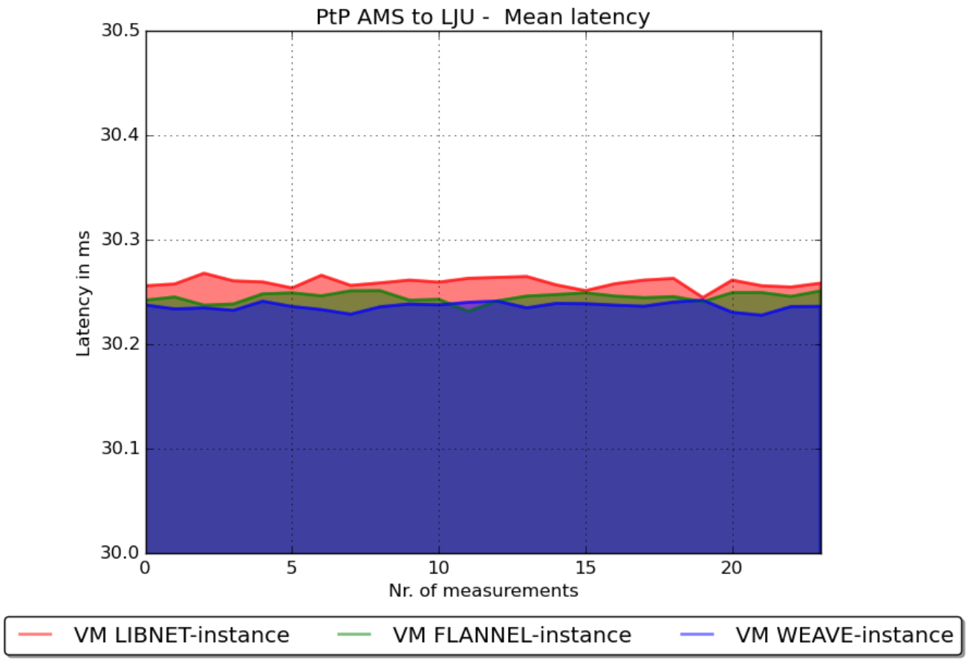
\includegraphics[scale=0.6]{img/ALL_AMS_LJU_MEANLAT.png}
   \caption{Single site VM measurements within three instances }
   \label{fig:ALL_AMS_LJU_MEANLAT}
\end{figure}

This means that later on, we can safely compare the overlay performances on the VMs which reside on different topology instances and possibly on different physical hosts. Based on the measurements above we can assume that all physical hosts within a site are identical in resources and utilization. Additionally, the absence of a day-night cycle and the insignificant amount of jitter indicates that there is little to no concurrent use of GTS taking place.

\subsection{Overlay performance} \label{synthetic}
Subsequently, we evaluate the general degradation of performance when introducing the overlay solutions into the equation. We started with the point-to-point measurements in the full mesh topology using \texttt{netperf}. In doing so, we have seen no significant differences in the jitter between the VMs and docker containers in any of the overlays. Any discrepancy within these results are small enough ($<$ 0.1 ms) to contribute to the fact that tests were ran subsequently to one another. When comparing overlay performances between each other, similar results are seen as portrayed in Table \ref{tab:PtP_Overlays_Latency}. Some outliers exist due to the limited amount of measurements that could be taken.
\\
\begin{table}[!ht]
\centering
\begin{tabular}{@{}lllll@{}}
\toprule
\textbf{Circuit} & \textbf{Instance} & \multicolumn{3}{c}{\textbf{In Milliseconds (ms)}} \\
\textbf{} & \textbf{} & \textit{\textbf{Min. Latency}} & \textit{\textbf{Mean Latency}} & \textit{\textbf{99th \% Latency}} \\ \midrule
AMS – MIL & Libnet & 36.3 & 36.5 & 37.0 \\
 & Weave & 36.2 & 36.5 & 37.0 \\
 & Flannel & 42.5 & 42.9 & 43.0 \\ \midrule
AMS – LJU & Libnet & 30.1 & 30.3 & 31.0 \\
 & Weave & 29.8 & 30.3 & 31 \\
 & Flannel & 29.8 & 30.3 & 31.0 \\ \midrule
AMS – BRA & Libnet & 17.6 & 17.7 & 18.0 \\
 & Weave & 17.4 & 17.7 & 18.0 \\
 & Flannel & 17.4 & 17.7 & 18.0 \\ \midrule
MIL – LJU & Libnet & 61.8 & 62.1 & 62.4 \\
\textit{} & Weave & 59.8 & 59.8 & 60.0 \\
\textit{} & Flannel & 55.6 & 55.8 & 56.0 \\ \midrule
\textit{MIL – BRA} & Libnet & 12.7 & 13.0 & 14.0 \\
\textit{} & Weave & 12.9 & 13.1 & 14.0 \\
\textit{} & Flannel & 12.9 & 13.1 & 14.0 \\ \midrule
\textit{BRA – LJU} & Libnet & 47.1 & 47.4 & 48.0 \\
\textit{} & Weave & 43.1 & 59.5 & 130.0 \\
\textit{} & Flannel & 43.1 & 43.3 & 44.0 \\ \bottomrule
\end{tabular}
\caption{Point-to-point latency measurements through the overlays }
\label{tab:PtP_Overlays_Latency}
\end{table}

Next, we saturate the link using \texttt{iperf}. Strangely enough, as figure \ref{fig:sub1} illustrates, we found that the TCP throughput in most cases resulted in the container out-performing the VM it is running on. The UDP throughput displayed in figure \ref{fig:sub2} shows a very different pattern. 

\begin{figure}[H]
\centering
\begin{subfigure}{.5\textwidth}
  \centering
  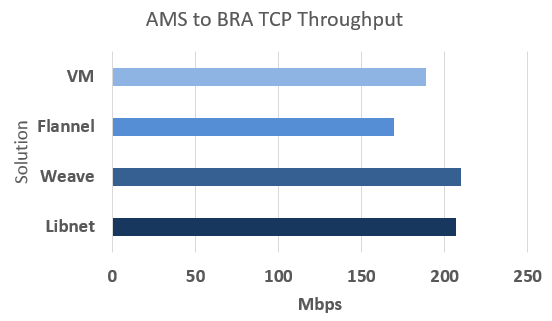
\includegraphics[scale=0.5]{img/PtP_All_TCP.PNG}
  \caption{TCP throughput}
  \label{fig:sub1}
\end{subfigure}%
\begin{subfigure}{.5\textwidth}
  \centering
  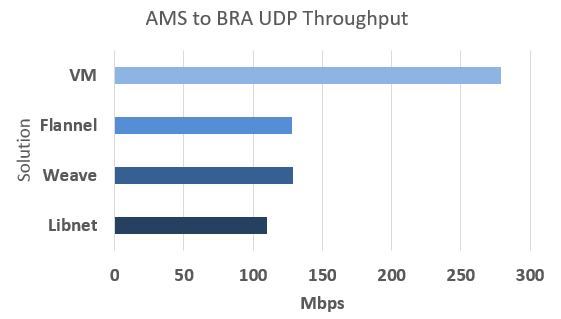
\includegraphics[scale=0.5]{img/PtP_All_UDP.PNG}
  \caption{UDP throughput}
  \label{fig:sub2}
\end{subfigure}
\caption{UDP and TCP throughput as measured on the Amsterdam - Bratislava circuit}
\label{fig:UDP_TCP_MSMT}
\end{figure}

The measured data indicates that the overlay solutions do not perform well during UDP testing. The full results of the experiment are presented in Appendix \ref{app:PtP}. Figure \ref{fig:UDP_TCP_MSMT} presents the results of the Amsterdam - Bratislava circuit. However, the measured anomalies are not specific to an individual circuit as is shown in Appendix \ref{app:PtP_through}. In some measurements the overlay outperforms the underlay whereas in other scenarios the opposite is true. 

Regarding the UDP throughput, Claassen examined similar behavior and hypothesized that the anomaly may be caused due to \texttt{iperf} consuming more CPU cycles for measuring the jitter of the UDP packets \cite{jorisclaassen2015}. However, in his work no anomalies were found regarding TCP throughput. This observation will be further explored in the discussion in Section \ref{discussion}. 

\subsection{Media streaming scenario}
After the point-to-point measurements, the performance of the overlays in a star-topology was evaluated by stressing a central node with a gradually increasing amount of concurrent sessions. In this scenario performance is defined by measuring the jitter on the link and the bit rate of the stream as measured on the client side. The streaming media measurements have been performed sequentially and within a single topology instance. 

Figure \ref{fig:sub3} presents the jitter results from the streaming test with a varying amount of Faban workers for the underlay and each of the overlays, specifically on the Bratislava - Amsterdam circuit. Little to no jitter is measured with a low amount of workers (e.g. one and three workers) is used as there is no real congestion on the link. In both cases the jitter remains below or around 0.5 milliseconds.  However, when the total amount of requested streams is increased to nine, artificial congestion is created on the 10 Mbps rate limited link. This inherently causes the jitter to increase. 

\begin{figure}[!ht]
\centering
\begin{subfigure}{.5\textwidth}
  \centering
  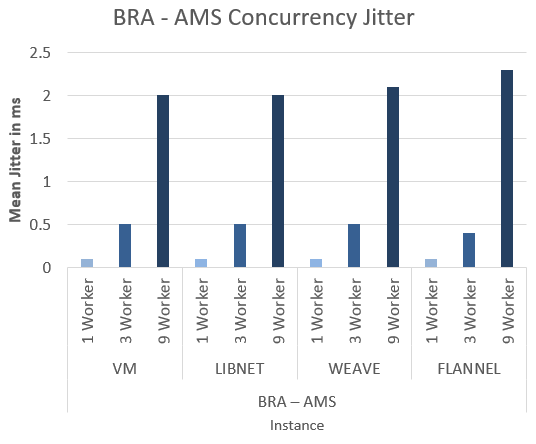
\includegraphics[scale=0.5]{img/All_Streaming_jitter.PNG}
  \caption{Jitter measurements}
  \label{fig:sub3}
\end{subfigure}%
\begin{subfigure}{.5\textwidth}
  \centering
  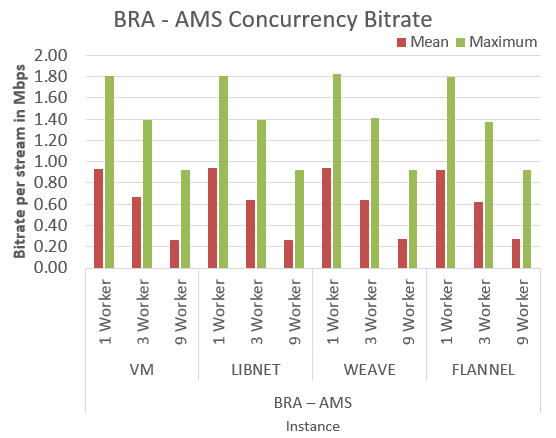
\includegraphics[scale=0.5]{img/All_Streaming_TP.PNG}
  \caption{Bit rate measurements}
  \label{fig:sub4}
\end{subfigure}
\caption{Concurrency measurements through the overlays and VM in the star topology}
\label{fig:PtP_All_TCP.PNG}
\end{figure}

During the stresstest the amount of jitter fluctuates between approximately 2 and 2.3 milliseconds. Figure \ref{fig:sub3} shows a slight increase in jitter for Weave and Flannel respectively, but this fluctuation is not significant and may be flattened out over the course of additional consecutive measurements. Furthermore, the difference in jitter between the virtual machines and the overlay solutions are not significant.

The measured values are below the recommendations from Cisco which state that a video stream should have less than 30 milliseconds of one way jitter \cite{szigeti_hattingh_2004}. Still, Claypool and Tanner show that even low amounts of jitter can have a high impact on the perceived quality of a video stream by end users \cite{claypool1999effects}. Client- and server-side buffering can be utilized to cope with slight increases in jitter.

As expected, the results from the bit rate evaluation indicate that bit rates per stream deteriorate when the amount of requesting clients increase. Figure \ref{fig:sub4} illustrates that the deterioration holds a very similar pattern between the underlay and the overlay solutions. There is no significant performance difference between a specific overlay solution and the underlay. Appendix \ref{app:stream} presents the full results of the media streaming scenario for each of the circuits as displayed in figure \ref{fig:stream_topology}.



%Conclusion
\section{Discussion} \label{discussion}
During the course of this project we measured the performance of various overlay solutions when implemented in a high latency environment. When starting out with the research, our hypothesis was that the overlay solutions would perform worse than the underlay in any given situation. This was based on the general notion that an overlay solution introduces an implicit performance overhead by adding another layer to the network. Additionally, as most overlay solutions now resort to in-kernel traffic handling, we did not expect the decrease in performance to be very large. 
\\\\
The results of the point-to-point UDP and TCP throughput measurements with \texttt{iperf} did not match our expectations. We saw irregular behavior whilst measuring TCP throughput. In most situations the overlay solution outperforms the underlay but sometimes the opposite is true. The measurements as presented in Appendix \ref{app:PtP_through} indicate that this behavior is not specific to an individual circuit. Similarly, we expected a small deterioration in performance whilst measuring the UDP throughput between containers in the overlays, but not with a margin of circa 100 to 150 Mbps. Interestingly enough, our results indicate that the anomalies regarding UDP throughput are constant. Regardless of the tested circuit a significant performance drop is seen. 

We are not the first ones to find anomalies in UDP throughput measurements. Claassen examined similar behavior in his paper regarding Docker network performance in a local environment \cite{jorisclaassen2015}. He hypothesized that the deterioration could be related to the way \texttt{iperf} functions with regards to its utilization of CPU cycles whilst measuring. Regarding the disappointing UDP throughput measured with \texttt{iperf}, Claassen's hypothesis holds. The fact that the streaming media tests also utilize UDP and do not show such losses does support the notion that this is indeed an \texttt{iperf} specific problem. Nevertheless, this does not explain why the overlay solutions outperform the underlay when TCP throughput is measured, which leads us to believe that this issue is specific to the GÉANT Testbeds Service. Further investigation is required.
\\\\
Due to the irregular results, we will presume the measurements in the point-to-point topology regarding UDP and TCP throughput are unreliable and as such, will not be used as a basis to form a conclusion. This decision does not impact the latency measurements however. These measurements consistently show that the underlay outperforms the overlay by a very small margin (below 1 millisecond). 
\\\\
With regards to latency, surprisingly enough, the latency measured within GTS resembled that of a non-shared environment. This is likely the case due to the fact that the environment is not intensively being used by other researchers. Because of this, we have been able to get unadulterated results regarding the performance of these overlays. As a consequence we have not experienced a level of congestion which would be expected in a real world scenario. It is possible that performing the experiments in an environment with a high(er) level of congestion would yield different results. This is especially true for the streaming media tests as in our current experiment we have only been able to see the effect of artificial congestion. 
\\\\
During the feasibility-check of the overlay solutions, we have noticed a difference in ease of setup between the different overlay technologies. Weave has proven to be the most inclusive package requiring no additional software to be installed while the other overlays require at least a separate key-value store. Considering there are no significant performance differences observed between the overlays -with regards to latency-, Weave could be considered the preferred solution within this specific environment. However, we feel that the choice for a certain solution is very specific to the use case of the network. For example, due to the fast deployment capabilities of Weave, the solution lends itself especially well for rapid prototyping. Flannel on the other hand is built to specifically to integrate with Google's Kubernetes orchestration tool which allows for the administration of very large clusters. Calico pursues a different model and is mainly aimed at high performance data center deployments. As a closing remark we think that the integration a solution offers with third party tools will be a hugely deciding factor when selecting a solution, as all of the solutions pursue a similar goal: interconnecting containers dispersed over multiple hosts, regardless of their physical location. 

%Conclusion
\section{Conclusion} \label{conclusion}
%Docker containers and container-based solutions in general are challenging virtual machines in cloud environments. An increasing number of companies are looking to either complement or even completely replace their virtual compute infrastructure with containers. Containers are lightweight and allow for a high density of deployed services. This transition is eased with the introduction of \texttt{libnetwork} in Docker, which allows for connecting geographically dispersed containers via means of either a native or a third party overlay network.

In this paper, we have evaluated the performance of various Docker overlay solutions in a high latency environment, and more specifically, in the GÉANT Testbeds Service. We assessed the native overlay driver included in \texttt{libnetwork} and third party solutions Flannel and Weave by means of a synthetic point-to-point benchmark and a streaming media application benchmark in a star topology. During the project, Calico was found to be infeasible to deploy in the GTS. We saw that the remaining solutions are very similar on a technical level and employ similar VXLAN tunneling techniques to connect containers. 
\\
\\
Our results indicate that the performance of the overlay solutions with regards to latency as well as jitter is very similar. The level of overhead introduced by the overlay can be considered almost negligible (in the range of 0.1 ms). The same behavior was found whilst measuring the performance of the overlays in the streaming media benchmark. All overlays exhibit similar performance, regardless of the amount of locations in the topology or clients requesting a stream. As such, we conclude that the native overlay driver performs equal to the evaluated third party solutions. Our point-to-point measurements show irregular behavior with regards to UDP and TCP throughput and require further investigation.
\\
\\
Taking all of the measurements into account, we conclude that geographic dispersion has no significant effect on either latency or jitter when evaluated in the GTS specifically. 

\subsection{Future work}
During the course of this project a GitHub repository\footnote{All created resources are available at \url{https://github.com/siemhermans/gtsperf}} has been maintained which is designed to make future deployments of the evaluated overlay solutions easier, particularly in GTS. However, although GTS is an excellent environment to test the synthetic performance of the overlays, it would be interesting to reconduct the performance analysis in a heavily shared environment (e.g. Amazon EC2 or Azure). This would require a slight modification of the provided scripts but would illustrate the effect of real world congestion on performance. Additionally, the measurements should be repeated in an environment which is less pressed for resources, in order to eliminate the CPU as a variable whilst measuring. With regards to the measured results, further investigation is required to identify the root cause of the anomalies seen in UDP and TCP throughput.  

With regards to the environment, the current measurements have been performed with a generic Infrastructure as a Service use case in mind. This means that the Docker containers have been deployed within virtual machines. In the future it would be interesting to see how the performance of the overlay solutions compares when the containers are deployed in a special container hypervisor like LXD \cite{ubuntulxd}. This would require a cloud provider to provide (near) bare metal provision resources. At this point in time, bare metal provisioning is not supported in GTS, however, it is a confirmed road-mapped functionality. Therefore, the GTS may potentially be used for this purpose in the future.


%Acknowledgements
\thispagestyle{acknowledgements}
\addcontentsline{toc}{section}{Acknowledgements}
\section*{Acknowledgements}
We would like to thank Dr. Paola Grosso for guiding us throughout the course of the project and for proofreading our initial proposal and the final report. Furthermore we would like to thank Susanne Naegele-Jackson for providing us (preliminary) access to the GÉANT Testbeds Service. Lastly we thank Fabio Farina and Nicolai Iliuha for their rapid response times regarding technical questions and feature requests with respect to the GTS infrastructure. 

\cleardoublepage
\begingroup

\addcontentsline{toc}{section}{References}
\bibliographystyle{unsrt}
\bibliography{bibliography}
\endgroup


%Appendices
\begin{appendices}
  \renewcommand\thetable{\thesection\arabic{table}}
  \renewcommand\thefigure{\thesection\arabic{figure}}
  \section{Dockerfile} \label{app:dockerfile}
  \begin{lstlisting}
# In order to write the logs to a file on the host, the container should be started as  'docker run --name perf_meas -v /data $IMAGE_ID'. The $IMAGE_ID is the ID of the image built with this Dockerfile. To view the logs, the following command should be run docker inspect -f '{{range .Mounts}}{{.Source}}{{end}}' $CONTAINER_NAME.

FROM ubuntu:14.04
MAINTAINER Siem Hermans, <siem.hermans@os3.nl>
LABEL version="1.0"
LABEL role="Performance measurement"

# Set timezone
ENV TZ=UTC

# Default to server mode with iperf TCP test

# Set correct directory
ENV dir /root
WORKDIR ${dir}

# Update sources & install essential tools  
RUN apt-get -qq update && apt-get install -yqq \
  wget \
  build-essential \
  git

# Pull and build testing tools (iperf3 & netperf)
RUN wget --no-check-certificate https://iperf.fr/download/iperf_3.0/iperf3_3.0.11-1_amd64.deb https://iperf.fr/download/iperf_3.0/libiperf0_3.0.11-1_amd64.deb
RUN dpkg -i libiperf0_3.0.11-1_amd64.deb iperf3_3.0.11-1_amd64.deb && rm libiperf0_3.0.11-1_amd64.deb iperf3_3.0.11-1_amd64.deb
RUN wget --no-check-certificate ftp://ftp.netperf.org/netperf/netperf-2.7.0.tar.gz && tar -xzvf netperf-2.7.0.tar.gz
RUN cd netperf-2.7.0 && ./configure --enable-demo=yes && make && make install && rm ../netperf-2.7.0.tar.gz

# Install netperf binaries and clean up directories
RUN mv -t /usr/bin netperf-2.7.0/src/netperf netperf-2.7.0/src/netserver && rm -rf netperf-2.7.0/

# Install iperf (2)
WORKDIR ${dir}
RUN wget --no-check-certificate http://heanet.dl.sourceforge.net/project/iperf/iperf-2.0.5.tar.gz 
RUN tar -xzvf iperf-2.0.5.tar.gz && cd iperf-2.0.5/src

# Patch iperf 2.0.5 in order to fix the 100% utilization bug when running iperf as a daemon
ADD scripts/nomaxcpu.patch ${dir}/iperf-2.0.5/src/nomaxcpu.patch
WORKDIR ${dir}/iperf-2.0.5/src/
RUN patch < nomaxcpu.patch
RUN cd .. && ./configure && make && make install && cp src/iperf /usr/bin/iperf

# Include netperf and iperf scripts
WORKDIR ${dir}
ADD scripts/perf_measurement.sh ${dir}/perf.sh
RUN chmod +x perf.sh

# Execute performance measurements
CMD ./perf.sh
#STOPSIGNAL SIGKILL

# Expose the default ports, statically linked (iperf TCP/UDP, iperf3, netperf)
EXPOSE 5001:5001 5002:5002 5201:5201 12865:12865
\end{lstlisting}
\newpage

\section{ Performance measurement script} \label{app:script}
\begin{lstlisting}
#!/bin/bash
# This script reads ENV variables set by the Dockerfile by default. To 
# override this behaviour, specify variables with docker run -e "VAR=value".
# Examples:
# docker run -e MODE="CLIENT" -e TEST="IPERF" -e TYPE="UDP" -e SRCSITE="AMS" -e DSTSITE="PRG" -e ADDRESS="172.17.0.2" -e OVERLAY="NONE" -v /data 18c2d4864eb3
# docker run -e MODE="SERVER" $IMAGE_ID

if [[ $MODE == "CLIENT" ]]; then
	# netperf measurement
	if [[ $TEST == "NETPERF" ]]; then
		# Generate timestamp (start)
		psstart=$(date +%Y%m%d%H%M%S)

		# Run performance measurement
		psresult=$(netperf -l 115 -H $ADDRESS -t UDP_RR -- -O min_latency,mean_latency,p99_latency,stddev_latency | tail -n 1 | awk '{$1=$1}1' OFS=",")

		# Generate timestamp (end)
		psend=$(date +%Y%m%d%H%M%S)

		# Write log to file
		echo $psstart","$psend","$OVERLAY","$SRCSITE","$DSTSITE","$psresult >> /data/'MSMT_'$SRCSITE'_'$DSTSITE'_'$TEST'_'$OVERLAY'.csv'

	elif [[ $TEST == "IPERF" ]]; then
		# Differentiate between TCP and UDP bandwidth test
		if [[ $TYPE == "UDP" ]]; then
			# Run performance measurement & write to CSV
			iperf -c $ADDRESS -u -p 5002 -b 1000M -y C -t 115 | tail -n 1 >> /data/'MSMT_'$SRCSITE'_'$DSTSITE'_'$TEST'_'$TYPE'_'$OVERLAY'.csv'

		elif [[ $TYPE == "TCP" ]]; then
			# Run performance measurement & write to CSV
			iperf -c $ADDRESS -p 5001 -y C -t 115 >> /data/'MSMT_'$SRCSITE'_'$DSTSITE'_'$TEST'_'$TYPE'_'$OVERLAY'.csv'
		fi
	fi

else
    # Enter server condition if the $MODE != client
	# Start netserver daemon
	netserver
	# Run iperf server as daemon mode (TCP and UDP respectively)
	iperf -s -D -p 5001
	iperf -s -u -p 5002
fi

\end{lstlisting}



\newpage
\section{Baseline Latency}\label{app:Baseline}

\begin{figure}[H]
\centering
  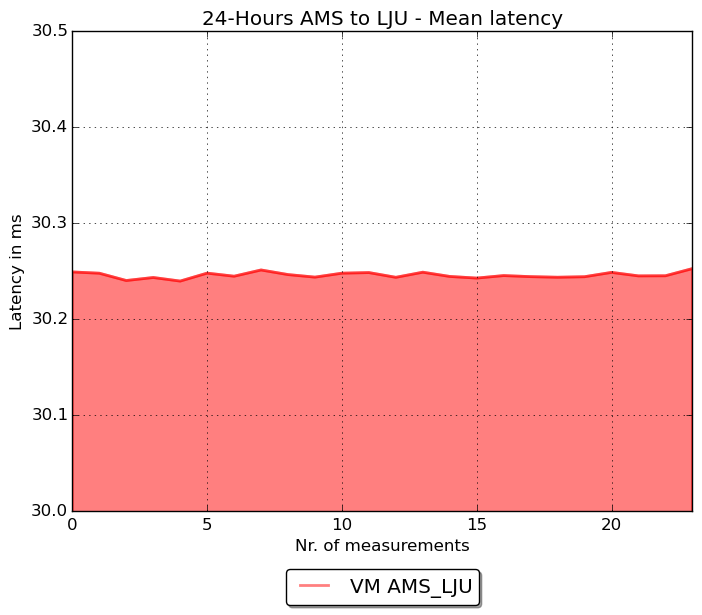
\includegraphics[scale=0.5]{img/24H_AMSLJU_MEANLAT.PNG}
  \caption{Mean Latency on all AMS to LJU circuits}
  \label{fig:sub5}
\end{figure}

\begin{figure}[H]
\centering
  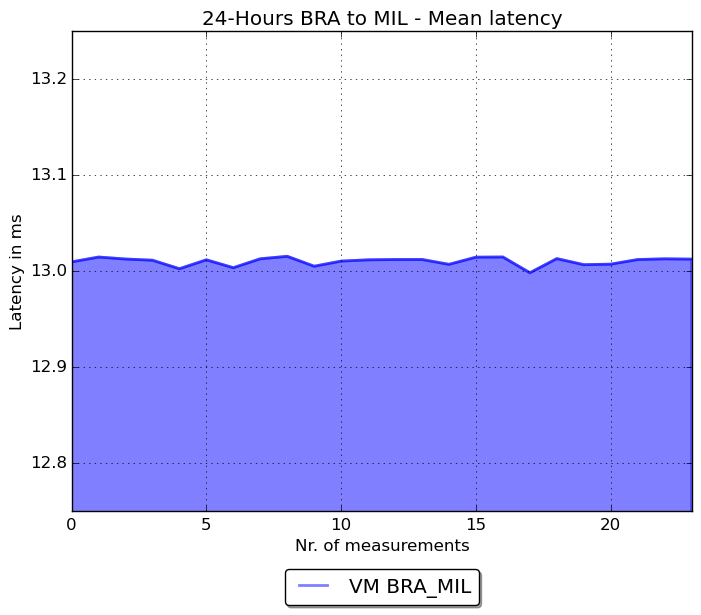
\includegraphics[scale=0.5]{img/24H_BRAMIL_MEANLAT.PNG}
  \caption{Mean Latency on all BRA to MIL circuits}
  \label{fig:sub6}
\end{figure}


\newpage
\section{ Point-to-Point Latency Measurements} \label{app:PtP}
% Please add the following required packages to your document preamble:
% \usepackage{booktabs}
% \usepackage{graphicx}

\setlength\LTleft{0pt}
\setlength\LTright{0pt}
\begin{longtable}{@{\extracolsep{\fill}}lllcccc@{}}
\toprule
\textbf{Instance} & \multicolumn{1}{l}{\textbf{Circuit}} & {\color[HTML]{333333} \textbf{Platform}} & \multicolumn{4}{c}{\textbf{In Milliseconds (ms)}} \\
\textbf{} & \textbf{} & {\color[HTML]{333333} \textbf{}} & \textit{\textbf{Min.}} & \textit{\textbf{Mean}} & \textit{\textbf{99th \%}} & \textit{\textbf{Stddev}} \\ \midrule
\textbf{Libnetwork} & \textit{AMS – MIL} & {\color[HTML]{333333} VM} & 36.3 & 36.5 & 37.0 & 0.1 \\
 &  & {\color[HTML]{333333} Docker} & 36.3 & 36.5 & 37.0 & 0.1 \\ \cmidrule(l){3-7} 
 &  & {\color[HTML]{333333} \textbf{Difference}} & 0.0 & 0.0 & 0.0 & 0.0 \\ \cmidrule(l){2-7} 
 & \textit{AMS – LJU} & {\color[HTML]{333333} VM} & 30.1 & 30.3 & 31.0 & 0.1 \\
 &  & {\color[HTML]{333333} Docker} & 30.1 & 30.3 & 31.0 & 0.1 \\ \cmidrule(l){3-7} 
 &  & {\color[HTML]{333333} \textbf{Difference}} & {\color[HTML]{CB0000} -0.1} & {\color[HTML]{CB0000} -0.1} & 0.0 & 0.0 \\ \cmidrule(l){2-7} 
 & \textit{AMS – BRA} & {\color[HTML]{333333} VM} & 17.5 & 17.7 & 18.0 & 0.1 \\
 &  & {\color[HTML]{333333} Docker} & 17.6 & 17.7 & 18.0 & 0.0 \\ \cmidrule(l){3-7} 
 &  & {\color[HTML]{333333} \textbf{Difference}} & {\color[HTML]{CB0000} -0.1} & {\color[HTML]{CB0000} -0.1} & 0.0 & 0.0 \\ \cmidrule(l){2-7} 
 & \textit{MIL – LJU} & {\color[HTML]{333333} VM} & 61.6 & 62.1 & 62.4 & 0.1 \\
 &  & {\color[HTML]{333333} Docker} & 61.8 & 62.1 & 62.4 & 0.1 \\ \cmidrule(l){3-7} 
 &  & {\color[HTML]{333333} \textbf{Difference}} & {\color[HTML]{CB0000} -0.2} & 0.0 & 0.0 & 0.0 \\ \cmidrule(l){2-7} 
 & \textit{MIL – BRA} & {\color[HTML]{333333} VM} & 12.7 & 13.0 & 14.0 & 0.1 \\
 &  & {\color[HTML]{333333} Docker} & 12.7 & 13.1 & 14.0 & 0.0 \\ \cmidrule(l){3-7} 
 &  & {\color[HTML]{333333} \textbf{Difference}} & 0.0 & {\color[HTML]{CB0000} -0.1} & 0.0 & 0.0 \\ \cmidrule(l){2-7} 
 & \textit{BRA – LJU} & {\color[HTML]{333333} VM} & 47.1 & 47.4 & 48.0 & 0.0 \\
 &  & {\color[HTML]{333333} Docker} & 47.2 & 47.4 & 48.0 & 0.0 \\ \cmidrule(l){3-7} 
 &  & {\color[HTML]{333333} \textbf{Difference}} & 0.0 & {\color[HTML]{CB0000} -0.1} & 0.0 & 0.0 \\ \midrule
\textbf{Weave} & \textit{AMS – MIL} & {\color[HTML]{333333} VM} & 36.1 & 36.4 & 37.0 & 0.0 \\
 &  & {\color[HTML]{333333} Docker} & 36.2 & 36.5 & 37.0 & 0.0 \\ \cmidrule(l){3-7} 
 &  & {\color[HTML]{333333} \textbf{Difference}} & {\color[HTML]{CB0000} -0.1} & {\color[HTML]{CB0000} -0.1} & 0.0 & 0.0 \\ \cmidrule(l){2-7} 
 & \textit{AMS – LJU} & {\color[HTML]{333333} VM} & 29.9 & 30.2 & 31.0 & 0.0 \\
 &  & {\color[HTML]{333333} Docker} & 29.8 & 30.3 & 31.0 & 0.0 \\ \cmidrule(l){3-7} 
 &  & {\color[HTML]{333333} \textbf{Difference}} & 0.0 & {\color[HTML]{CB0000} -0.1} & 0.0 & 0.0 \\ \cmidrule(l){2-7} 
 & \textit{AMS – BRA} & {\color[HTML]{333333} VM} & 17.4 & 17.7 & 18.0 & 0.1 \\
 & \textit{} & {\color[HTML]{333333} Docker} & 17.4 & 17.7 & 18.0 & 0.1 \\ \cmidrule(l){3-7} 
 & \textit{} & {\color[HTML]{333333} \textbf{Difference}} & {\color[HTML]{CB0000} -0.1} & 0.0 & 0.0 & 0.0 \\ \cmidrule(l){2-7} 
 & \textit{MIL – LJU} & {\color[HTML]{333333} VM} & 59.6 & 59.8 & 60.0 & 0.1 \\
 & \textit{} & {\color[HTML]{333333} Docker} & 59.6 & 59.8 & 60.0 & 0.1 \\ \cmidrule(l){3-7} 
 & \textit{} & {\color[HTML]{333333} \textbf{Difference}} & 0.0 & {\color[HTML]{CB0000} -0.1} & 0.0 & 0.0 \\ \cmidrule(l){2-7} 
 & \textit{MIL – BRA} & {\color[HTML]{333333} VM} & 12.8 & 13.0 & 14.0 & 0.1 \\
 &  & {\color[HTML]{333333} Docker} & 12.9 & 13.1 & 14.0 & 0.1 \\ \cmidrule(l){3-7} 
 &  & {\color[HTML]{333333} \textbf{Difference}} & {\color[HTML]{CB0000} -0.1} & {\color[HTML]{CB0000} -0.1} & 0.0 & 0.0 \\ \cmidrule(l){2-7} 
 & \textit{BRA – LJU} & {\color[HTML]{333333} VM} & 43.0 & 43.3 & 44.0 & 0.1 \\
 & \textit{} & {\color[HTML]{333333} Docker} & 43.1 & 59.5 & 130.0 & 0.1 \\ \cmidrule(l){3-7} 
 & \textit{} & {\color[HTML]{333333} \textbf{Difference}} & {\color[HTML]{CB0000} -0.2} & {\color[HTML]{CB0000} -16.2} & {\color[HTML]{CB0000} -86.0} & 0.0 \\ \midrule
\textbf{Flannel} & \textit{AMS – MIL} & {\color[HTML]{333333} VM} & 42.4 & 42.8 & 43.0 & 0.0 \\
 & \textit{} & {\color[HTML]{333333} Docker} & 42.5 & 42.9 & 43.0 & 0.0 \\ \cmidrule(l){3-7} 
 & \textit{} & {\color[HTML]{333333} \textbf{Difference}} & {\color[HTML]{CB0000} -0.1} & {\color[HTML]{CB0000} -0.1} & 0.0 & 0.0 \\ \cmidrule(l){2-7} 
 & \textit{AMS – LJU} & {\color[HTML]{333333} VM} & 29.8 & 30.2 & 31.0 & 0.0 \\
 & \textit{} & {\color[HTML]{333333} Docker} & 29.8 & 30.3 & 31.0 & 0.0 \\ \cmidrule(l){3-7} 
 & \textit{} & {\color[HTML]{333333} \textbf{Difference}} & 0.1 & {\color[HTML]{CB0000} -0.1} & 0.0 & 0.0 \\ \cmidrule(l){2-7} 
 & \textit{AMS – BRA} & {\color[HTML]{333333} VM} & 17.3 & 17.7 & 18.0 & 0.0 \\
 & \textit{} & {\color[HTML]{333333} Docker} & 17.4 & 17.7 & 18.0 & 0.0 \\ \cmidrule(l){3-7} 
 &  & {\color[HTML]{333333} \textbf{Difference}} & {\color[HTML]{CB0000} -0.1} & 0.0 & 0.0 & 0.0 \\ \cmidrule(l){2-7} 
 & \textit{MIL – LJU} & {\color[HTML]{333333} VM} & 55.5 & 55.8 & 56.0 & 0.0 \\
 & \textit{} & {\color[HTML]{333333} Docker} & 55.6 & 55.8 & 56.0 & 0.0 \\
 & \textit{} & {\color[HTML]{333333} \textbf{Difference}} & {\color[HTML]{CB0000} -0.1} & {\color[HTML]{CB0000} -0.1} & 0.0 & 0.0 \\ \cmidrule(l){2-7} 
 & \textit{MIL – BRA} & {\color[HTML]{333333} VM} & 12.8 & 13.0 & 14.0 & 0.0 \\
 & \textit{} & {\color[HTML]{333333} Docker} & 12.9 & 13.1 & 14.0 & 0.0 \\ \cmidrule(l){3-7} 
 & \textit{} & {\color[HTML]{333333} \textbf{Difference}} & {\color[HTML]{CB0000} -0.1} & {\color[HTML]{CB0000} -0.1} & 0.0 & 0.0 \\ \cmidrule(l){2-7} 
 & \textit{BRA – LJU} & {\color[HTML]{333333} VM} & 43.1 & 43.4 & 44.0 & 0.0 \\
 &  & {\color[HTML]{333333} Docker} & 43.1 & 43.4 & 44.0 & 0.0 \\ \cmidrule(l){3-7} 
 &  & {\color[HTML]{333333} \textbf{Difference}} & {\color[HTML]{CB0000} -0.1} & 0.0 & 0.0 & 0.0 \\ \bottomrule
\end{longtable}

\newpage
\section{ Point-to-Point Throughput Measurements} \label{app:PtP_through}

\setlength\LTleft{0pt}
\setlength\LTright{0pt}
\begin{longtable}{@{\extracolsep{\fill}}lclcc@{}}
\toprule
\textbf{Instance} & \multicolumn{1}{l}{\textbf{Circuit}} & {\color[HTML]{333333} \textbf{Platform}} & \multicolumn{2}{l}{\textbf{Throughput in Mbps}} \\
\textbf{} & \textbf{} & {\color[HTML]{333333} \textbf{}} & \textit{\textbf{TCP}} & \textit{\textbf{UDP}} \\ \midrule
\textbf{Libnetwork} & \textit{AMS – MIL} & {\color[HTML]{333333} VM} & 150.7 & 231.6 \\
 &  & {\color[HTML]{333333} Docker} & 213.2 & 110.6 \\ \cmidrule(l){3-5} 
 &  & {\color[HTML]{333333} \textbf{Difference}} & {\color[HTML]{CB0000} -62.5} & {\color[HTML]{009901} 121.1} \\ \cmidrule(l){2-5} 
 & \textit{AMS – LJU} & {\color[HTML]{333333} VM} & 152.5 & 223.3 \\
 &  & {\color[HTML]{333333} Docker} & 165.3 & 110.0 \\ \cmidrule(l){3-5} 
 &  & {\color[HTML]{333333} \textbf{Difference}} & {\color[HTML]{CB0000} -12.8} & {\color[HTML]{009901} 113.3} \\ \cmidrule(l){2-5} 
 & \textit{AMS – BRA} & {\color[HTML]{333333} VM} & 148.9 & 225.5 \\
 &  & {\color[HTML]{333333} Docker} & 207.1 & 109.9 \\ \cmidrule(l){3-5} 
 &  & {\color[HTML]{333333} \textbf{Difference}} & {\color[HTML]{CB0000} -58.2} & {\color[HTML]{009901} 115.6} \\ \cmidrule(l){2-5} 
 & \textit{MIL – LJU} & {\color[HTML]{333333} VM} & 127.4 & 238.4 \\
 &  & {\color[HTML]{333333} Docker} & 128.3 & 130.1 \\ \cmidrule(l){3-5} 
 &  & {\color[HTML]{333333} \textbf{Difference}} & {\color[HTML]{CB0000} -0.8} & {\color[HTML]{009901} 108.3} \\ \cmidrule(l){2-5} 
 & \textit{MIL – BRA} & {\color[HTML]{333333} VM} & 181.2 & 254.5 \\
 &  & {\color[HTML]{333333} Docker} & 167.0 & 129.2 \\ \cmidrule(l){3-5} 
 &  & {\color[HTML]{333333} \textbf{Difference}} & {\color[HTML]{009901} 14.2} & {\color[HTML]{009901} 125.4} \\ \cmidrule(l){2-5} 
 & \textit{BRA – LJU} & {\color[HTML]{333333} VM} & 158.8 & 226.7 \\
 &  & {\color[HTML]{333333} Docker} & 133.7 & 111.8 \\ \cmidrule(l){3-5} 
 &  & {\color[HTML]{333333} \textbf{Difference}} & {\color[HTML]{009901} 25.0} & {\color[HTML]{009901} 114.8} \\ \midrule
\textbf{Weave} & \textit{AMS – MIL} & {\color[HTML]{333333} VM} & 179.0 & 272.8 \\
 &  & {\color[HTML]{333333} Docker} & 243.0 & 130.5 \\ \cmidrule(l){3-5} 
 &  & {\color[HTML]{333333} \textbf{Difference}} & {\color[HTML]{CB0000} -64.0} & {\color[HTML]{009901} 142.2} \\ \cmidrule(l){2-5} 
 & \textit{AMS – LJU} & {\color[HTML]{333333} VM} & 189.2 & 249.9 \\
 &  & {\color[HTML]{333333} Docker} & 201.6 & 129.3 \\ \cmidrule(l){3-5} 
 &  & {\color[HTML]{333333} \textbf{Difference}} & {\color[HTML]{CB0000} -12.4} & {\color[HTML]{009901} 120.6} \\ \cmidrule(l){2-5} 
 & \textit{AMS – BRA} & {\color[HTML]{333333} VM} & 188.5 & 255.4 \\
 & \textit{} & {\color[HTML]{333333} Docker} & 209.8 & 128.9 \\ \cmidrule(l){3-5} 
 & \textit{} & {\color[HTML]{333333} \textbf{Difference}} & {\color[HTML]{CB0000} -21.2} & {\color[HTML]{009901} 126.5} \\ \cmidrule(l){2-5} 
 & \textit{MIL – LJU} & {\color[HTML]{333333} VM} & 131.7 & 255.3 \\
 & \textit{} & {\color[HTML]{333333} Docker} & 161.5 & 128.5 \\ \cmidrule(l){3-5} 
 & \textit{} & {\color[HTML]{333333} \textbf{Difference}} & {\color[HTML]{9A0000} -29.8} & {\color[HTML]{009901} 126.8} \\ \cmidrule(l){2-5} 
 & \textit{MIL – BRA} & {\color[HTML]{333333} VM} & 188.5 & 261.0 \\
 &  & {\color[HTML]{333333} Docker} & 217.9 & 130.4 \\ \cmidrule(l){3-5} 
 &  & {\color[HTML]{333333} \textbf{Difference}} & {\color[HTML]{CB0000} -29.3} & {\color[HTML]{009901} 130.6} \\ \cmidrule(l){2-5} 
 & \textit{BRA – LJU} & {\color[HTML]{333333} VM} & 149.9 & 229.0 \\
 & \textit{} & {\color[HTML]{333333} Docker} & 43.9 & 17.2 \\ \cmidrule(l){3-5} 
 & \textit{} & {\color[HTML]{333333} \textbf{Difference}} & {\color[HTML]{009901} 106.0} & {\color[HTML]{009901} 211.8} \\ \midrule
\textbf{Flannel} & \textit{AMS – MIL} & {\color[HTML]{333333} VM} & 177.1 & 271.9 \\
 & \textit{} & {\color[HTML]{333333} Docker} & 187.5 & 126.9 \\ \cmidrule(l){3-5} 
 & \textit{} & {\color[HTML]{333333} \textbf{Difference}} & {\color[HTML]{CB0000} -10.4} & {\color[HTML]{009901} 145.0} \\ \cmidrule(l){2-5} 
 & \textit{AMS – LJU} & {\color[HTML]{333333} VM} & 180.2 & 268.1 \\
 & \textit{} & {\color[HTML]{333333} Docker} & 225.6 & 128.3 \\ \cmidrule(l){3-5} 
 & \textit{} & {\color[HTML]{333333} \textbf{Difference}} & {\color[HTML]{CB0000} -45.4} & {\color[HTML]{009901} 139.8} \\ \cmidrule(l){2-5} 
 & \textit{AMS – BRA} & {\color[HTML]{333333} VM} & 187.2 & 267.0 \\
 & \textit{} & {\color[HTML]{333333} Docker} & 169.8 & 127.8 \\ \cmidrule(l){3-5} 
 &  & {\color[HTML]{333333} \textbf{Difference}} & {\color[HTML]{009901} 17.4} & {\color[HTML]{009901} 139.2} \\ \cmidrule(l){2-5} 
 & \textit{MIL – LJU} & {\color[HTML]{333333} VM} & 142.2 & 278.8 \\
 & \textit{} & {\color[HTML]{333333} Docker} & 210.7 & 131.9 \\
 & \textit{} & {\color[HTML]{333333} \textbf{Difference}} & {\color[HTML]{CB0000} -68.6} & {\color[HTML]{009901} 146.9} \\ \cmidrule(l){2-5} 
 & \textit{MIL – BRA} & {\color[HTML]{333333} VM} & 194.2 & 254.0 \\
 & \textit{} & {\color[HTML]{333333} Docker} & 211.3 & 130.6 \\ \cmidrule(l){3-5} 
 & \textit{} & {\color[HTML]{333333} \textbf{Difference}} & {\color[HTML]{CB0000} -17.1} & {\color[HTML]{009901} 123.4} \\ \cmidrule(l){2-5} 
 & \textit{BRA – LJU} & {\color[HTML]{333333} VM} & 151.7 & 243.2 \\
 &  & {\color[HTML]{333333} Docker} & 214.6 & 110.0 \\ \cmidrule(l){3-5} 
 &  & {\color[HTML]{333333} \textbf{Difference}} & {\color[HTML]{CB0000} -63.0} & {\color[HTML]{333333} 133.2} \\ \bottomrule
\end{longtable}

\newpage
\section{ Streaming media measurements} \label{app:stream}
\begin{table}[!ht]
\small
\centering
\resizebox{\textwidth}{!}{%
\begin{tabular}{@{}lcccccc@{}}
\toprule
\multicolumn{1}{c}{} & \textbf{Circuit} & \textbf{Workers} & \multicolumn{3}{c}{\textbf{Bit rate (Kbps)}} & \textbf{Jitter (ms)} \\
\rowcolor[HTML]{FFFFFF} 
 & \textbf{} & \textbf{} & \textit{\textbf{Min.}} & \textit{\textbf{Mean}} & \textit{\textbf{Max.}} & \textbf{} \\ \midrule
\textbf{VM} & \textit{BRA – AMS} & 1 & 112.09 & 957.59 & 1853.68 & 0.08 \\ 
\textbf{} & \textit{} & 3 & 69.59 & 681.23 & 1429.48 & 0.45 \\
\textbf{} & \textit{} & 9 & 41.18 & 272.17 & 944.11 & 2.10 \\
\textbf{} & \textit{BRA – MIL} & 1 & 111.19 & 955.46 & 1854.89 & 0.09 \\
\textbf{} & \textit{} & 3 & 69.13 & 671.21 & 1426.39 & 0.55 \\
\textbf{} & \textit{} & 9 & 39.40 & 273.45 & 932.24 & 2.00 \\
\textbf{} & \textit{BRA – LJU} & 1 & 111.33 & 948.15 & 1851.54 & 0.09 \\
\textbf{} & \textit{} & 3 & 68.99 & 670.25 & 1421.54 & 0.49 \\
\textbf{} & \textit{} & 9 & 40.49 & 268.25 & 919.55 & 1.92 \\ \midrule
\textbf{Weave} & \textit{BRA – AMS} & 1 & 113.20 & 958.70 & 1851.37 & 0.10 \\
\textbf{} & \textit{} & 3 & 68.93 & 654.39 & 1422.14 & 0.47 \\
\textbf{} & \textit{} & 9 & 40.17 & 270.41 & 941.41 & 2.14 \\
\textbf{} & \textit{BRA – MIL} & 1 & 108.47 & 948.94 & 1849.74 & 0.09 \\
\textbf{} & \textit{} & 3 & 70.52 & 648.69 & 1409.49 & 0.49 \\
\textbf{} & \textit{} & 9 & 39.35 & 272.28 & 935.86 & 1.86 \\
\textbf{} & \textit{BRA – LJU} & 1 & 109.74 & 944.86 & 1834.43 & 0.09 \\
\textbf{} &  & 3 & 66.23 & 650.13 & 1414.70 & 0.47 \\
\textbf{} &  & 9 & 41.09 & 269.38 & 928.17 & 2.29 \\ \midrule
\textbf{Libnetwork} & \textit{BRA – AMS} & 1 & 113.79 & 963.13 & 1868.45 & 0.06 \\
\textbf{} & \textit{} & 3 & 67.78 & 659.49 & 1445.72 & 0.46 \\
\textbf{} & \textit{} & 9 & 40.22 & 277.33 & 941.81 & 2.01 \\
\textbf{} & \textit{BRA – MIL} & 1 & 109.93 & 949.45 & 1799.31 & 0.06 \\
\textbf{} & \textit{} & 3 & 69.98 & 650.90 & 1416.16 & 0.48 \\
\textbf{} & \textit{} & 9 & 38.96 & 273.05 & 934.06 & 1.74 \\
\textbf{} & \textit{BRA – LJU} & 1 & 112.00 & 948.27 & 1833.70 & 0.08 \\
\textbf{} & \textit{} & 3 & 72.79 & 642.49 & 1426.46 & 0.50 \\
\textbf{} &  & 9 & 37.44 & 271.10 & 917.75 & 1.98 \\ \midrule
\textbf{Flannel} & \textit{BRA – AMS} & 1 & 109.87 & 947.41 & 1837.20 & 0.11 \\
\textbf{} & \textit{} & 3 & 64.24 & 632.10 & 1402.66 & 0.40 \\
\textbf{} & \textit{} & 9 & 40.33 & 274.38 & 944.66 & 2.28 \\
\textbf{} & \textit{BRA – MIL} & 1 & 105.56 & 947.71 & 1829.12 & 0.13 \\
\textbf{} & \textit{} & 3 & 66.53 & 621.74 & 1427.34 & 0.45 \\
\textbf{} & \textit{} & 9 & 40.10 & 272.09 & 928.99 & 1.91 \\
\textbf{} & \textit{BRA – LJU} & 1 & 110.88 & 946.26 & 1844.49 & 0.10 \\
\textbf{} & \textit{} & 3 & 62.97 & 623.68 & 1467.22 & 0.46 \\
\textbf{} &  & 9 & 41.26 & 267.24 & 916.67 & 2.43 \\ \midrule
\end{tabular}
}
\end{table}
  
\end{appendices}


\end{document}